% !TEX TS-program = xelatex
% !BIB program = bibtex
% !TEX encoding = UTF-8 Unicode

\documentclass[
  twoside,
  openright,
  degree    = master,               % degree = master | doctor
  language  = chinese,              % language = chinese | english
  fontset   = template,             % fontset = default | template | system | overleaf
  watermark = true,                 % watermark = true | false
  doi       = true,                 % doi = true | false
]{ntuthesis}

% !TeX root = ./main.tex

% --------------------------------------------------
% 資訊設定（Information Configs）
% --------------------------------------------------

\ntusetup{
  university*   = {National Taiwan University},
  university    = {國立臺灣大學},
  college       = {工學院},
  college*      = {College of Engineering},
  institute     = {工程科學與海洋工程研究所},
  institute*    = {Institute of Engineering Science and Ocean Engineering},
  title         = {應用知識圖譜注意力網路於食譜推薦之效能評估與可解釋性研究},
  title*        = {Performance Evaluation and Explainability Study of Knowledge Graph Attention Network for Recipe Recommendation},
  author        = {廖健合},
  author*       = {Jian-He Liao},
  ID            = {R12525066},
  advisor       = {張瑞益},
  advisor*      = {RaY-I Chang},
  % date          = {2026-04-30},         % 若註解掉，則預設為當天
  % oral-date     = {2026-07-30},         % 若註解掉，則預設為當天
  % DOI           = {10.5566/NTU2026XXXXX},
  keywords      = {知識圖譜, 注意力機制, 食譜推薦, 深度學習, 協同過濾, 可解釋性},
  keywords*     = {Knowledge Graph, Attention Mechanism, Recipe Recommendation, Deep Learning, Collaborative Filtering, Explainability},
}

% --------------------------------------------------
% 加載套件（Include Packages）
% --------------------------------------------------

\usepackage[numbers,sort&compress]{natbib} % 參考文獻（數字格式，與 abbrv 相容）
\usepackage{amsmath, amsthm, amssymb}   % 數學環境
\usepackage{ulem, CJKulem}              % 下劃線、雙下劃線與波浪紋效果
\usepackage{booktabs}                   % 改善表格設置
\usepackage{multirow}                   % 合併儲存格
\usepackage{diagbox}                    % 插入表格反斜線
\usepackage{array}                      % 調整表格高度
\usepackage{longtable}                  % 支援跨頁長表格
\usepackage{paralist}                   % 列表環境
\usepackage{subcaption}                 % 子圖
\usepackage{enumitem}                   % 進階列表
\usepackage{bm}                         % 粗體數學符號
\usepackage{tabularx}                   % 自適應寬度表格
\usepackage{float}                      % 強制定位表格 [H]
\usepackage{xcolor}                     % 顏色支援
\usepackage{pifont}                     % 特殊符號 (ding)
\usepackage{standalone}                 % 獨立輸出
\usepackage{tikz}                       % 繪圖
\usetikzlibrary{positioning, arrows.meta, shapes.geometric, fit, backgrounds, shadows}
% --------------------------------------------------
% 套件設定（Packages Settings）
% --------------------------------------------------

\begin{document}

% 封面與口試審定
% Cover and Verification Letter
\makecover                          % 論文封面（Cover）
% \makeverification                   % 口試委員審定書（Verification Letter）

% 致謝與論文摘要
% Acknowledgement and Abstract
\input{front/acknowledgement}       % 致謝（Acknowledgement）
% !TeX root = ../main.tex

\begin{abstract}

隨著網路食譜平台的蓬勃發展，使用者面臨嚴重的資訊過載問題，亟需有效的推薦系統協助探索潛在偏好的食譜內容。本研究以知識圖譜注意力網路 (Knowledge Graph Attention Network, KGAT) 為核心，在 Food.com 食譜推薦資料集上進行系統性的效能評估與可解釋性研究。

本研究的主要貢獻包含三個面向。首先，透過消融實驗，顯示圖神經網路的訊息傳播深度是影響推薦效能的重要因素：三層架構 ($L{=}3$) 的 HR@20 達 0.8775，較單層架構 ($L{=}1$) 提升逾 29\%，較最強的基準方法 LightGCN 更提升達 31\%，全面超越 BPR-MF、LightGCN 及 NFM 等基準方法。其次，發現在淺層架構 ($L{=}1$) 下，引入知識圖譜反而因雜訊稀釋協同過濾訊號而導致效能下降，此發現與近期文獻~\cite{zhang2024kg4receval}所觀察到之知識圖譜貢獻非必然正面的結論相呼應，為知識圖譜整合策略提供了重要啟示。最後，本研究以 500 位使用者為基礎，對三種不同深度的 KGAT 模型（$L{=}1$、$L{=}2$、$L{=}3$）進行跨模型 Fidelity 量化評估。在最佳效能模型 KGAT-3L 中，278 位使用者成功萃取解釋路徑（覆蓋率 55.6\%），其中 94.2\% 的路徑 Fidelity$^+$ 大於零，支持注意力權重標記了對預測有貢獻的關鍵邊。進一步的路徑類型分析發現，直接連接路徑的忠實度最高（Avg $F^+=0.0494$，$F^- \approx 0$），而 KG 語意路徑的充分性忠實度持續偏低（$F^-=0.2449$），暗示深層模型的決策可能已將部分知識圖譜結構資訊壓縮進分散式嵌入中，使得顯式圖譜路徑無法完整涵蓋模型的決策依據。

\end{abstract}

\begin{abstract*}

With the rapid growth of online recipe platforms, users face severe information overload, necessitating effective recommender systems to help discover recipes matching their preferences. This study systematically evaluates the performance and explainability of the Knowledge Graph Attention Network (KGAT) on the Food.com recipe recommendation dataset.

Our contributions are threefold. First, through ablation experiments, we show that the message propagation depth of graph neural networks is an important factor for recommendation performance: the three-layer architecture ($L{=}3$) achieves an HR@20 of 0.8775, representing a 29\% improvement over the single-layer architecture ($L{=}1$) and a 31\% improvement over the strongest baseline LightGCN, substantially outperforming baseline methods including BPR-MF, LightGCN, and NFM. Second, we discover that incorporating the knowledge graph in the shallow architecture ($L{=}1$) paradoxically degrades performance, as noise dilutes the collaborative filtering signals---a finding consistent with recent work by Zhang et al.~\cite{zhang2024kg4receval} questioning the unconditional benefit of knowledge graphs in recommender systems---providing important insights for knowledge graph integration strategies. Third, using a cohort of 500 users, we conduct a cross-model Fidelity evaluation across three KGAT depths ($L{=}1$, $L{=}2$, $L{=}3$). In the best-performing KGAT-3L model, 278 users yield explanation paths (coverage 55.6\%), of which 94.2\% exhibit positive Fidelity$^+$, supporting that attention weights identify edges contributing to predictions. Path-type analysis further reveals that direct connection paths achieve the highest fidelity (Avg $F^+=0.0494$, $F^- \approx 0$), while KG semantic paths exhibit persistently poor sufficiency fidelity ($F^-=0.2449$), suggesting that deep models may partly compress knowledge graph structural information into distributed representations where explicit graph paths cannot fully capture the model's decision evidence.

\end{abstract*}              % 摘要（Abstract）

% 生成目錄與符號列表
% Contents of Tables and Denotation
\maketableofcontents                % 目錄（Table of Contents）
\makelistoffigures                  % 圖目錄（List of Figures）
\makelistoftables                   % 表目錄（List of Tables）
% !TeX root = ../main.tex

\begin{denotation}[4cm]

\item[$\mathcal{G}$]{
  協同知識圖譜 (Collaborative Knowledge Graph, CKG)
}

\item[$\mathcal{U}$]{
  使用者集合 (User Set)
}

\item[$\mathcal{V}$]{
  物品集合 (Item Set)
}

\item[$\mathcal{E}$]{
  實體集合 (Entity Set)
}

\item[$\mathcal{R}$]{
  關係集合 (Relation Set)
}

\item[$\bm{e}_u, \bm{e}_v$]{
  使用者 $u$ 與物品 $v$ 的嵌入向量 (Embedding Vector)
}

\item[$\bm{e}_r$]{
  關係 $r$ 的嵌入向量
}

\item[$d$]{
  嵌入維度 (Embedding Dimension)
}

\item[$L$]{
  圖神經網路的訊息傳播層數 (Number of Propagation Layers)
}

\item[$\alpha_{ij}$]{
  節點 $i$ 對鄰居節點 $j$ 的注意力權重 (Attention Weight)
}

\item[$\mathcal{N}_i$]{
  節點 $i$ 的鄰居集合 (Neighborhood Set)
}

\item[$\hat{y}_{uv}$]{
  使用者 $u$ 對物品 $v$ 的預測偏好分數
}

\item[$p_{uv}$]{
  使用者 $u$ 對物品 $v$ 的預測機率 (亦即 $\sigma(\hat{y}_{uv})$)
}

\item[$\mathcal{L}_{\text{BPR}}$]{
  貝葉斯個人化排序損失函數 (BPR Loss)
}

\item[HR@$K$]{
  命中率，Top-$K$ 推薦清單中包含真實正樣本的比例
}

\item[NDCG@$K$]{
  歸一化折損累計增益，衡量推薦排序品質
}

\item[P@$K$]{
  精確率，Top-$K$ 推薦清單中正確推薦的比例
}

\item[$S$]{
  解釋路徑萃取框架中所選定的解釋邊集合 (Explanatory Subgraph)
}

\item[$F^+, F^-$]{
  必要性 (Necessity) 與充分性 (Sufficiency) 忠實度量化指標 (Fidelity)
}

\end{denotation}
            % 符號列表（Denotation）

% 論文內容
% Contents of Thesis
\mainmatter
% !TeX root = ../main.tex

\chapter{緒論}

\section{研究背景與動機}

隨著網際網路的蓬勃發展與行動裝置的普及，線上食譜平台（如 Food.com、Allrecipes 等）累積了數以百萬計的食譜內容與使用者互動紀錄。面對如此龐大的資訊量，使用者往往難以從海量的選項中找到真正符合自身口味偏好、飲食需求或烹飪條件的食譜。這種「資訊過載」(Information Overload) 問題催生了推薦系統 (Recommender System) 的廣泛應用與深入研究~\cite{su2009survey}。

傳統的推薦方法大多奠基於協同過濾 (Collaborative Filtering, CF) 技術~\cite{koren2009matrix}，透過分析使用者與物品之間的歷史互動矩陣來預測潛在偏好。然而，此類方法在面對資料稀疏性 (Data Sparsity) 與冷啟動 (Cold-start) 問題時，往往暴露出其架構上的根本限制——當使用者與物品的互動紀錄極度匱乏時，協同過濾模型便無法有效地捕捉潛在的偏好模式。

為突破上述瓶頸，學術界開始嘗試將知識圖 (Knowledge Graph, KG) 引入推薦系統~\cite{wang2018ripplenet, wang2019kgcn}。知識圖透過「頭實體——關係——尾實體 $(h, r, t)$」的三元組 (Triplet) 結構，構建出一個龐大且高度互連的語義網路。以食譜推薦為例，一道食譜可透過「包含食材」、「屬於菜系」、「適合場合」等多種關係，與其他食譜或屬性實體產生豐富的語義連結。這種結構化的背景知識能有效緩解資料稀疏性問題，並賦予推薦系統對食譜內涵的深層語義理解能力。

在此背景下，圖神經網路 (Graph Neural Networks, GNNs)~\cite{kipf2017gcn, velickovic2018gat} 成為融合知識圖與推薦系統的強力工具。其中，Wang 等人~\cite{wang2019kgat} 提出的知識圖注意力網路 (Knowledge Graph Attention Network, KGAT)，透過端到端的學習方式，將使用者與物品的互動矩陣和知識圖融合為一個協同知識圖 (Collaborative Knowledge Graph, CKG)，並運用注意力機制在多跳 (Multi-hop) 路徑上進行遞迴式的嵌入傳播，明確地模擬了高階連接性 (High-order Connectivity)，在推薦準確度上取得了突破性的進展。

然而，隨著模型架構複雜度的提升，圖神經網路推薦系統逐漸淪為難以解讀的「黑盒子」(Black-box)。使用者僅能看到推薦結果，卻無從得知系統為何做出此推薦。這種不透明性在食譜推薦場景中尤為關鍵——使用者可能存在過敏原限制、特殊飲食偏好或營養考量，若系統無法解釋推薦依據，將嚴重影響使用者的信任程度與採納意願~\cite{zhang2020explainable}。因此，如何在追求高準確度的同時，賦予推薦系統可解釋性 (Explainability)，使其能清楚闡述「為何推薦此食譜」，已成為當前研究的重要課題。

\section{現有方法之不足與研究缺口}

儘管 KGAT 在多個基準資料集上展現了優異的推薦效能，回顧現有文獻仍可辨識出以下三個尚未被充分探索的研究缺口：

\begin{enumerate}[leftmargin=2em]
  \item \textbf{領域適用性之空白：}KGAT 原論文~\cite{wang2019kgat}僅在 Amazon-Book、Yelp2018 及 Last-FM 三個電商或娛樂領域的基準資料集上進行驗證，尚未涉及食譜此種語義結構高度密集的領域。食譜知識圖具有與商品知識圖截然不同的圖拓撲特性——例如少數食材（如 \texttt{chicken}、\texttt{sugar}）往往連結數千筆食譜，形成高度偏斜的度分佈——這些特性可能對模型行為產生未預期的影響。

  \item \textbf{深度效應與模組貢獻分析仍有不足：}既有 KGAT 相關研究在報告實驗結果時，通常僅呈現最佳深度配置的效能數值，而較少系統性比較從 L=1 到 L=3 的效能變化趨勢。即使部分研究會討論注意力機制或知識圖的作用，其模組拆解多半侷限於有限設定，尚不足以完整釐清不同傳播深度下各元件的邊際貢獻如何變化。

  \item \textbf{深層 GNN 可解釋性驗證之匱乏：}多數可解釋性研究停留於定性案例展示，或僅在淺層模型（$L \leq 2$）上進行小樣本的忠實度 (Fidelity) 評估~\cite{yuan2022explainability}。隨著傳播深度增加，注意力路徑在多層非線性轉換後的 Fidelity 究竟如何演變，目前缺乏在深層 GNN（$L{=}3$）上的大規模 Fidelity 量化驗證。此外，傳統 Fidelity 指標在邊移除或保留過程中可能引發的分佈偏移 (Distribution Shift) 問題~\cite{agarwal2024fidelity}，亦鮮少在推薦場景中被討論。
\end{enumerate}

\section{研究目的}

基於上述研究缺口，本研究以 KGAT 為核心架構，在 Food.com 食譜推薦資料集上進行系統性的效能評估與可解釋性研究。具體而言，本研究旨在回答以下三個研究問題：

\begin{itemize}[leftmargin=2em]
  \item \textbf{RQ1：圖神經網路深度與知識圖整合如何影響推薦效能？} \\
  本研究將比較不同傳播深度下 KGAT 的效能變化，並在淺層設定下初步拆解注意力機制與知識圖的影響，並與 BPR-MF~\cite{rendle2009bpr}、LightGCN~\cite{he2020lightgcn}、NFM~\cite{he2017nfm} 等基準方法進行對比，以分析深度與知識整合在食譜推薦場景中的實際作用。
  \item \textbf{RQ2：不同傳播深度下，模型的訓練行為與泛化能力有何差異？} \\
    分析從 $L{=}1$ 到 $L{=}3$ 的深度變化對模型收斂速度、過擬合 (Overfitting) 現象及最終效能的影響。
  \item \textbf{RQ3：基於注意力機制的解釋路徑是否忠實地反映了模型的決策邏輯？} \\
    建構一套完整的可解釋性評估框架，以 500 位使用者為基礎，對三種不同深度的 KGAT 模型（$L{=}1$、$L{=}2$、$L{=}3$）進行跨模型 Fidelity 量化評估，驗證注意力路徑對模型預測的實際影響力。
\end{itemize}

\section{研究貢獻}

本研究的貢獻包含以下三點：

\begin{enumerate}[leftmargin=2em]
  \item \textbf{深度效應之實證分析：}本研究在 Food.com 食譜推薦場景下，比較了 $L{=}1$ 到 $L{=}3$ 的傳播深度對 KGAT 推薦效能的影響，呈現深度變化與效能提升之間的具體關聯，並支持高階連接性在此類知識圖推薦任務中的重要性。
  \item \textbf{淺層 KG 整合效果之觀察：}本研究在淺層設定 $L{=}1$ 下觀察到，引入知識圖未必必然帶來效能提升；相反地，在特定圖結構條件下，知識圖可能引入額外雜訊，進而稀釋原有的協同過濾訊號。此結果提醒我們，知識整合的效果可能與圖結構特性及傳播深度密切相關。
  \item \textbf{深層模型之 Fidelity 量化分析：}本研究建立從注意力路徑萃取到 Fidelity 量化的分析流程，並在 $L{=}1$、$L{=}2$、$L{=}3$ 三種深度的 KGAT 模型上，以 500 位使用者為基礎進行系統性的跨模型 Fidelity 比較評估。結果顯示，不同深度與路徑類型呈現不同的必要性與充分性分布，說明基於注意力的解釋雖具分析價值，但其解釋品質仍需結合量化指標審慎檢驗。
\end{enumerate}

\section{論文架構}

本論文共分為五章，各章節內容安排如下：

\textbf{第一章~緒論：}介紹研究背景、動機、前人缺口與三個核心研究問題。

\textbf{第二章~文獻探討：}回顧推薦系統的技術演進，包含協同過濾、圖神經網路、知識圖增強推薦及可解釋推薦等相關文獻，並以方法差異比較表歸納研究缺口。

\textbf{第三章~研究方法：}詳述本研究所採用的 KGAT 模型架構、知識圖建構流程、損失函數設計，以及基於 Fidelity 指標的可解釋性評估框架。

\textbf{第四章~實驗設計與結果分析：}呈現完整的實驗結果，包含主要效能對比、消融實驗分析及可解釋性評估結果，並對各項發現進行深入討論。

\textbf{第五章~結論與未來研究方向：}總結研究成果，回應三個研究問題，討論研究限制，並提出未來可改進的方向。

% !TeX root = ../main.tex

\chapter{文獻探討}

本章針對本研究所涉及的四個核心技術領域進行系統性的文獻回顧：推薦系統的基礎方法、圖神經網路的理論框架、知識圖譜在推薦系統中的應用，以及可解釋推薦的最新發展。最後，以方法差異比較表歸納現有方法之不足與本研究之定位。

\section{推薦系統}

推薦系統根據其核心原理可分為三大類：基於內容的過濾 (Content-based Filtering)、協同過濾 (Collaborative Filtering) 以及混合式方法~\cite{su2009survey}。

\subsection*{協同過濾}

協同過濾是目前應用最為廣泛的推薦技術，其核心假設為「擁有相似歷史行為的使用者，在未來也將展現相似的偏好」。矩陣分解 (Matrix Factorization)~\cite{koren2009matrix} 作為協同過濾的經典實現，將龐大的使用者-物品互動矩陣分解為兩個低秩矩陣的乘積，藉此在潛在空間中捕捉使用者與物品的隱含特徵。

Rendle 等人~\cite{rendle2009bpr} 提出的貝葉斯個人化排序 (Bayesian Personalized Ranking, BPR) 進一步優化了矩陣分解在隱式回饋 (Implicit Feedback) 場景下的效能。BPR 採用成對排序損失 (Pairwise Ranking Loss)，假設使用者對已互動物品的偏好應高於未互動物品，並透過最大化貝葉斯後驗機率來學習最佳的排序模型。BPR-MF 至今仍被廣泛用作推薦系統研究的基準方法之一。

\subsection*{特徵互動模型}

為了克服純協同過濾在特徵利用上的不足，Rendle~\cite{rendle2010fm} 提出了因子分解機 (Factorization Machines, FM)，能夠自動學習特徵之間的二階交互作用。He 與 Chua~\cite{he2017nfm} 進一步提出 Neural Factorization Machines (NFM)，以神經網路取代 FM 中的線性二階交互，透過 Bi-Interaction Pooling 層學習更複雜的非線性特徵組合。然而，FM 系列方法將每一次互動視為獨立樣本，無法建模使用者與物品之間的高階拓撲關聯。

\section{圖神經網路 (Graph Neural Networks)}

圖神經網路 (GNNs) 是一類專門處理圖結構資料的深度學習模型，其核心思想是透過「訊息傳遞」(Message Passing)~\cite{gilmer2017mpnn} 機制，讓每個節點聚合其鄰居的特徵資訊，從而學習結構感知的節點表示。

\subsection*{圖卷積網路 (GCN)}

Kipf 與 Welling~\cite{kipf2017gcn} 提出的圖卷積網路 (Graph Convolutional Network, GCN) 是圖神經網路的里程碑之作。GCN 在頻譜域上對圖信號進行卷積操作，等價於在空間域上對節點的一階鄰居進行加權聚合。每一層 GCN 可擴展節點的感受野 (Receptive Field)，使得 $L$ 層的 GCN 能夠捕捉到 $L$-hop 範圍內的結構資訊。

\subsection*{圖注意力網路 (GAT)}

Veli\v{c}kovi\'{c} 等人~\cite{velickovic2018gat} 提出的圖注意力網路 (Graph Attention Network, GAT) 引入了自注意力 (Self-attention) 機制，使得模型在聚合鄰居資訊時，能夠根據鄰居節點的重要性動態分配不同的權重。相較於 GCN 中固定的拉普拉斯歸一化權重，GAT 的注意力機制提供了更靈活且具適應性的聚合策略，同時也為模型的可解釋性提供了天然的支持——高注意力權重的邊可被視為模型的重要決策依據。

\subsection*{LightGCN}

He 等人~\cite{he2020lightgcn} 在推薦系統的場景中提出了 LightGCN，主張移除 GCN 中的特徵轉換矩陣與非線性啟動函數，僅保留最核心的鄰居聚合操作。LightGCN 透過對不同層的嵌入進行加權求和，在大幅簡化模型複雜度的同時，反而取得了優異的推薦效能。此方法證明了在推薦場景中，過於複雜的非線性轉換可能反而阻礙了協同過濾訊號的傳遞。

\subsection*{深層 GNN 的挑戰：過度平滑與訓練穩定性}

隨著圖神經網路層數的增加，節點嵌入在反覆的鄰居聚合後會逐漸趨於一致，導致所謂的「過度平滑」(Over-smoothing) 現象~\cite{li2018deeper}。Zhao 與 Akoglu~\cite{zhao2020pairnorm} 提出的 PairNorm 透過保持節點嵌入的成對距離，在一定程度上緩解了此問題。Rong 等人~\cite{rong2020dropedge} 則提出 DropEdge，在每次訓練迭代中隨機移除一定比例的邊，類似於 Dropout 的正則化效果，有效提升了深層圖神經網路的訓練穩定性。這些研究為深層 GNN 推薦模型的可行性提供了技術基礎，但在知識圖譜推薦場景中的應用仍有待探索。

\section{知識圖譜與推薦系統之結合}

知識圖譜是一種以「頭實體——關係——尾實體」$(h, r, t)$ 三元組形式儲存結構化知識的語義網路。在推薦系統中引入知識圖譜，能為物品提供豐富的語義屬性描述，有效緩解資料稀疏性與冷啟動問題。

\subsection*{嵌入式方法}

嵌入式方法~\cite{wang2019cke} 將知識圖譜嵌入 (Knowledge Graph Embedding) 與推薦模型聯合訓練，利用如 TransE~\cite{bordes2013transe} 等平移模型預先學習實體與關係的低維向量表示，再將其作為推薦模型的附加特徵。這類方法雖然有效，但通常忽略了圖譜中的高階連接結構。

\subsection*{傳播式方法}

傳播式方法直接在知識圖譜的拓撲結構上進行遞迴的訊息傳播。RippleNet~\cite{wang2018ripplenet} 提出「偏好傳播」(Preference Propagation) 的概念，透過使用者偏好沿知識圖譜的漣漪狀擴散，自動發現使用者與候選物品之間的潛在連結。KGCN~\cite{wang2019kgcn} 則借鑑了 GCN 的訊息傳遞架構，對知識圖譜中物品的鄰居進行遞迴聚合。

\subsection*{多跳推理式方法}

近年來，部分研究進一步結合強化學習 (Reinforcement Learning) 在知識圖譜上進行多跳推理，賦予推薦以可解釋的路徑。Xian 等人~\cite{xian2019kgpolicy} 提出的 PGPR 將推薦問題轉化為知識圖譜上的路徑搜尋任務，訓練一個策略網路 (Policy Network) 學習從使用者出發、沿 KG 邊移動到達目標物品的最佳路徑。這類方法雖天然具備可解釋性（推薦路徑即為解釋），但其推理效率受限於搜尋空間的指數增長，且可能犧牲了推薦準確度。

\subsection*{KGAT：協同知識圖譜上的注意力傳播}

Wang 等人~\cite{wang2019kgat} 提出的 KGAT 是目前知識圖譜推薦系統中最具代表性的作品之一。KGAT 的核心創新在於：(1) 構建協同知識圖譜 (CKG)，將使用者-物品互動圖與物品知識圖譜統一為一個異質圖 (Heterogeneous Graph)；(2) 設計關係感知的注意力機制 (Relation-aware Attention)，根據三元組 $(h, r, t)$ 中不同關係的語義，動態調整鄰居聚合的權重；(3) 透過多層的注意力傳播 (Attentive Embedding Propagation)，明確建模高階連接性。原論文在 Amazon-Book、Yelp2018 及 Last-FM 三個基準資料集上，均取得了超越當時所有基準方法的效能。

然而，KGAT 原論文在以下面向仍留有研究空間：首先，驗證領域僅涵蓋電商與娛樂場景，對於如食譜此種語義結構高度密集的領域未有著墨；其次，原文僅報告最佳深度配置結果，未進行逐層的深度消融分析；最後，原文未對注意力路徑的忠實度進行量化驗證，使得其「內在可解釋性」的主張缺乏實證支撐。

\subsection*{知識增強推薦與大型語言模型之對比}

近年來，大型語言模型 (Large Language Models, LLMs) 也開始被應用於推薦系統。Gao 等人~\cite{gao2023chat} 提出的 Chat-REC 嘗試將對話式 LLM 與推薦系統結合，利用自然語言理解能力來增強使用者-物品的語義匹配。然而，LLM 為主的推薦方法在處理大規模結構化圖譜資訊上仍面臨效率瓶頸——LLM 需要將圖結構線性化為文字序列，在此過程中不可避免地損失高階拓撲資訊。相較之下，GNN 能夠在圖的原生結構上直接進行訊息傳播，更適合建模知識圖譜中複雜的多跳關聯。本研究選擇以 GNN 為技術路線，正是基於此結構化建模優勢。

\section{可解釋性推薦 (Explainable Recommendation)}

推薦系統的可解釋性旨在使系統能夠向使用者解釋「為何推薦此物品」~\cite{zhang2020explainable}，從而提升使用者的信任度、滿意度與決策效率。

\subsection*{圖神經網路的事後解釋}

隨著圖神經網路在推薦系統中的廣泛應用，針對 GNN 的可解釋性研究也日益受到關注。GNNExplainer~\cite{ying2019gnnexplainer} 是該領域的開創性工作，它透過學習一個邊遮罩 (Edge Mask)，尋找對模型預測結果影響最大的子圖結構。然而，GNNExplainer 屬於事後解釋 (Post-hoc Explanation) 方法，需要額外的優化過程，且可能面臨生成的解釋並非完全忠實於模型內部推理邏輯的問題~\cite{yuan2022explainability}。

\subsection*{基於注意力的內在可解釋性}

相較於事後解釋，基於注意力機制的路徑萃取提供了一條更為直接的可解釋性途徑。KGAT 與 GAT 架構天然地在正向傳播過程中計算每條邊的注意力權重 $\alpha_{ij}$，這些權重反映了模型在聚合訊息時對各鄰居的關注程度。透過追蹤高權重邊，可從使用者出發，沿著圖譜的拓撲結構一步步追溯到推薦物品，形成一條語義連貫的解釋路徑（例如：使用者 $\rightarrow$ 歷史食譜 $\rightarrow$ 共同食材 $\rightarrow$ 推薦食譜）。

\subsection*{忠實度 (Fidelity) 評估}

忠實度是衡量解釋品質最核心的量化指標，它衡量生成的解釋與模型真實決策邏輯之間的契合程度~\cite{yuan2022explainability}。常用的忠實度指標包含：

\begin{itemize}[leftmargin=2em]
  \item \textbf{Fidelity$^+$（必要性）：}移除解釋路徑上的邊後，若模型預測機率顯著下降，則證明這些邊對預測具有不可替代性。
  \item \textbf{Fidelity$^-$（充分性）：}僅保留解釋路徑上的邊，若模型預測機率幾乎不變，則證明這些邊已涵蓋支撐決策的充分資訊。
\end{itemize}

理想的解釋應同時具備高 Fidelity$^+$（標記了關鍵邊）與低 Fidelity$^-$（涵蓋了完整資訊）。然而，Agarwal 等人~\cite{agarwal2024fidelity} 指出，傳統基於遮罩 (masking) 的 Fidelity 評估方法可能因引入分佈偏移 (Distribution Shift) 而導致失真——模型在訓練期間從未見過如此「殘缺」的輸入圖結構，因此在評估時的預測行為可能偏離其正常運作模式。此問題在深層 GNN 中可能更加嚴重，但目前相關文獻甚少在推薦場景中加以討論。

此外，目前多數研究在 Fidelity 評估時面臨樣本量不足、僅在淺層模型上驗證等限制，深層模型（$L \geq 3$）的可解釋性驗證仍為一個尚未被充分探索的研究方向。本研究即針對此缺口，在三種不同深度的 KGAT 模型（$L{=}1$、$L{=}2$、$L{=}3$）上，以 500 位使用者為基礎進行系統性的 Fidelity 比較評估。

\section{現有方法之比較與研究缺口}

表~\ref{tab:method_comparison} 彙整了本研究所涉及的主要方法在五個關鍵維度上的差異，以凸顯本研究的獨特定位。

\begin{table}[htbp]
  \centering
  \caption{現有方法之差異比較}
  \label{tab:method_comparison}
  \resizebox{\textwidth}{!}{%
  \begin{tabular}{l ccccc}
    \toprule
    方法 & 使用 KG & 可解釋性 & Fidelity 量化 & 深度消融 & 食譜領域 \\
    \midrule
    BPR-MF~\cite{rendle2009bpr}        & \ding{55} & \ding{55} & \ding{55} & \ding{55} & \ding{55} \\
    LightGCN~\cite{he2020lightgcn}     & \ding{55} & \ding{55} & \ding{55} & \ding{55} & \ding{55} \\
    RippleNet~\cite{wang2018ripplenet}  & \ding{51} & 部分     & \ding{55} & \ding{55} & \ding{55} \\
    KGCN~\cite{wang2019kgcn}           & \ding{51} & \ding{55} & \ding{55} & \ding{55} & \ding{55} \\
    PGPR~\cite{xian2019kgpolicy}       & \ding{51} & \ding{51} & \ding{55} & \ding{55} & \ding{55} \\
    GNNExplainer~\cite{ying2019gnnexplainer} & \ding{55} & \ding{51} & 小規模  & \ding{55} & \ding{55} \\
    KGAT~\cite{wang2019kgat}           & \ding{51} & 潛在     & \ding{55} & \ding{55} & \ding{55} \\
    \midrule
    \textbf{本研究}                     & \ding{51} & \ding{51} & 系統性  & \textbf{\ding{51}} & \textbf{\ding{51}} \\
    \bottomrule
  \end{tabular}%
  }
\end{table}

綜觀上表，可以辨識出三個核心研究缺口：(1) 目前仍缺乏在食譜推薦領域系統性驗證 KGAT 效能與適用性的研究；(2) 既有研究對傳播深度的比較仍不充分，尚不足以清楚釐清深度變化對知識圖譜推薦效能的影響；(3) 深層 GNN 模型之注意力路徑忠實度仍缺乏較具規模的量化驗證。本研究即針對上述缺口提供具體的實證分析；其中，對深度效應提供了較完整的比較，對模組貢獻與可解釋性則提供初步而有系統的量化觀察。
% !TeX root = ../main.tex

\chapter{研究方法}

本章詳述本研究所採用的模型架構與評估方法，包含系統整體架構、食譜知識圖譜的建構流程、KGAT 模型的數學形式化、訓練策略，以及基於忠實度指標的可解釋性評估框架。

\section{系統架構}

本研究之系統架構可分為四個階段：(1) 資料預處理與知識圖譜建構：將 Food.com 原始資料轉化為結構化的協同知識圖譜；(2) 模型訓練：在協同知識圖譜上訓練 KGAT 模型，學習使用者與食譜的高品質嵌入表示；(3) 推薦生成：基於學習到的嵌入，為每位使用者生成 Top-$K$ 推薦清單；(4) 可解釋性評估：透過注意力路徑萃取與忠實度指標量化，驗證推薦結果的可解釋性。

\begin{figure}[htbp]
  \centering
  \includestandalone{figures/system_architecture}
  \caption{系統架構示意圖}
  \label{fig:system_architecture}
\end{figure}

\section{資料預處理與知識圖譜建構}

\subsection*{Food.com 資料集}

本研究採用 Food.com 食譜推薦資料集~\cite{majumder2019foodcom}，該資料集包含使用者對食譜的評分紀錄、食譜的詳細屬性（包含食材、標籤、營養成分等）。經過預處理後，我們將其轉化為隱式回饋形式——即僅保留使用者是否與食譜互動過的二元訊號，不區分評分高低。

\subsection*{協同知識圖譜 (CKG) 建構}

遵循 KGAT~\cite{wang2019kgat} 的設計理念，我們將使用者-食譜互動圖與食譜知識圖譜統一為一個協同知識圖譜 $\mathcal{G}$。具體而言：

\begin{figure}[htbp]
  \centering
  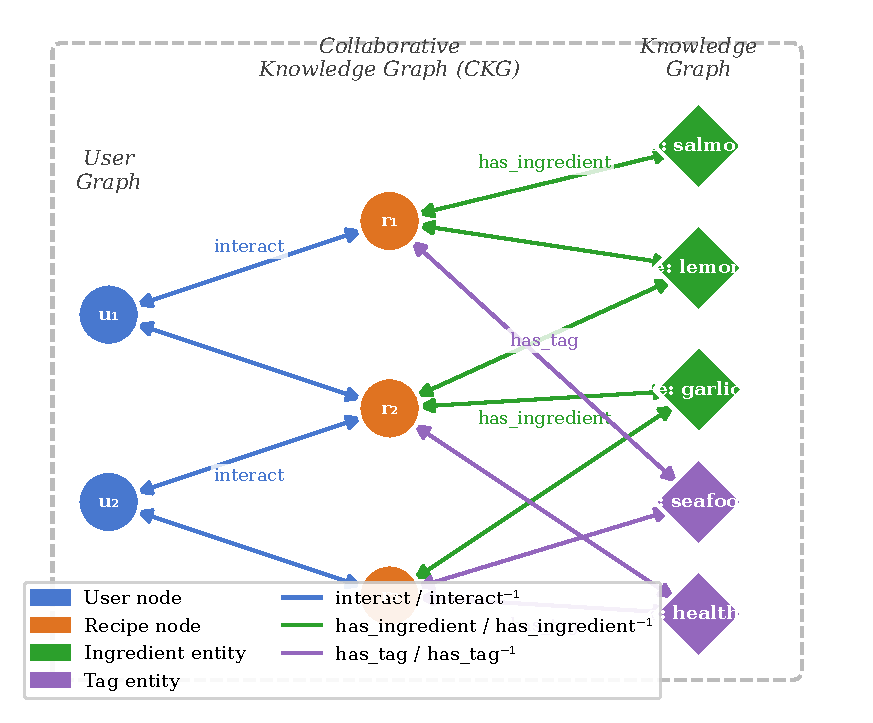
\includegraphics[width=0.82\linewidth]{figures/fig_ckg_schema.pdf}
  \caption{協同知識圖譜 (CKG) 架構示意：整合使用者-食譜互動圖與食譜知識圖譜，包含互動、食材與標籤三類關係邊。}
  \label{fig:ckg_schema}
\end{figure}

\begin{enumerate}[leftmargin=2em]
  \item \textbf{互動圖：}若使用者 $u$ 在訓練集中曾與食譜 $v$ 互動（例如收藏或評分），則建立邊 $(u, \text{interact}, v)$。測試集中的互動不納入 CKG，以避免資訊洩漏。
  \item \textbf{食譜屬性圖：}將食譜的標籤（如 \texttt{breakfast}、\texttt{chicken}、\texttt{weeknight}）與食材等屬性作為知識圖譜中的實體節點，並建立對應的關係邊，共形成食材（\texttt{has\_ingredient}）與標籤（\texttt{has\_tag}）兩類知識關係。例如，「食譜 A 包含食材 chicken」表示為三元組 $(v_A, \text{has\_ingredient}, e_\text{chicken})$。
  \item \textbf{反向邊擴充：}為確保訊息的雙向傳播，對每條邊 $(h, r, t)$ 均建立其反向邊 $(t, r^{-1}, h)$。
\end{enumerate}

最終建構的 CKG 包含使用者節點、食譜節點與屬性實體節點三類節點，以及互動關係與知識關係兩類邊。

\subsection*{超級節點修剪 (Super-node Pruning)}
  \label{sec:supernode_pruning}

在建構知識圖譜三元組之前，本研究先對高頻屬性實體進行超級節點修剪，以避免過度通用的節點在訊息傳播過程中引入大量雜訊路徑。

\begin{itemize}[leftmargin=2em]
  \item \textbf{食材超級節點：}統計所有食材的出現頻率後，移除出現頻率排名前 0.5\% 的高頻食材，以及根據先驗常識加入的基礎調味料（如 \texttt{salt}、\texttt{water}、\texttt{butter}、\texttt{sugar}、\texttt{eggs} 等）。兩部分取聯集後，共排除 74 個食材實體（詳細清單見附錄~\ref{app:preprocessing}）。這些食材出現在絕大多數食譜中，若納入 KG 將成為連結數萬節點的超級節點，其嵌入幾乎無法攜帶具有區辨力的語義資訊。
  \item \textbf{標籤超級節點：}統計所有標籤的出現頻率後，移除出現頻率排名前 50 的高頻標籤（如 \texttt{easy}、\texttt{healthy}、\texttt{main-dish} 等），這些標籤涵蓋面過廣，無法有效區分食譜的特色屬性。
\end{itemize}

此設計決策的理論依據在於：超級節點因與大量節點相連，其在 GNN 訊息傳播中相當於一個「資訊匯流點」，會造成鄰近節點的嵌入趨於相似（過度平滑）~\cite{li2018deeper}，並嚴重放大 §\ref{sec:kg_ablation} 所述的「淺層知識圖譜資訊汙染」效應。修剪後的知識圖譜保留語義區辨力強的屬性實體，使得實體間的關聯更能反映食譜的獨特風味特色。

\section{知識圖譜注意力網路 (KGAT)}

KGAT 模型由三個核心元件構成：嵌入層 (Embedding Layer)、注意力傳播層 (Attentive Propagation Layer) 與預測層 (Prediction Layer)。

\subsection*{嵌入層}

嵌入層將 CKG 中的每個節點與每條關係映射至 $d$ 維的稠密向量空間。對於節點 $i \in \mathcal{U} \cup \mathcal{V} \cup \mathcal{E}$，其初始嵌入為 $\bm{e}_i^{(0)} \in \mathbb{R}^d$；對於關係 $r \in \mathcal{R}$，其嵌入為 $\bm{e}_r \in \mathbb{R}^d$。

\subsection{Relation-Aware Attention 機制}

KGAT 的核心創新在於其關係感知的注意力機制。對於 CKG 中的一條邊 $(h, r, t)$，注意力分數的計算過程如下：

首先，計算三元組的原始注意力分數：
\begin{equation}
  \pi(h, r, t) = (\bm{W}_r \bm{e}_t)^\top \tanh \left( \bm{W}_r \bm{e}_h + \bm{e}_r \right)
  \label{eq:attention_raw}
\end{equation}
其中 $\bm{W}_r \in \mathbb{R}^{d' \times d}$ 為關係 $r$ 的轉換矩陣。此公式考慮了頭實體 $h$、關係 $r$ 與尾實體 $t$ 之間的語義相容性。

接著，透過 Softmax 歸一化得到最終的注意力權重：
\begin{equation}
  \alpha_{(h,r,t)} = \frac{\exp\left(\pi(h,r,t)\right)}{\sum_{(h,r',t') \in \mathcal{N}_h} \exp\left(\pi(h,r',t')\right)}
  \label{eq:attention_softmax}
\end{equation}
其中 $\mathcal{N}_h$ 表示節點 $h$ 在 CKG 中的所有鄰居三元組集合。

\subsection{Bi-Interaction 聚合機制}

在計算注意力權重後，KGAT 採用雙向互動 (Bi-Interaction) 聚合機制來更新節點表示。對於目標節點 $h$ 的第 $l$ 層嵌入更新：

首先計算注意力加權的鄰居聚合向量：
\begin{equation}
  \bm{e}_{\mathcal{N}_h}^{(l)} = \sum_{(h,r,t) \in \mathcal{N}_h} \alpha_{(h,r,t)} \cdot \bm{e}_t^{(l-1)}
  \label{eq:neighbor_agg}
\end{equation}

接著，透過加和（加性）與逐元素相乘（乘性）兩種互動方式組合：
\begin{equation}
  \bm{e}_h^{(l)} = \text{LeakyReLU}\left(\bm{W}_1^{(l)} \left(\bm{e}_h^{(l-1)} + \bm{e}_{\mathcal{N}_h}^{(l)}\right) + \bm{W}_2^{(l)} \left(\bm{e}_h^{(l-1)} \odot \bm{e}_{\mathcal{N}_h}^{(l)}\right)\right)
  \label{eq:bi_interaction}
\end{equation}
其中 $\bm{W}_1^{(l)}, \bm{W}_2^{(l)} \in \mathbb{R}^{d_l \times d_{l-1}}$ 為可學習的權重矩陣，$\odot$ 表示逐元素相乘 (Hadamard Product)。加性部分捕捉節點自身特徵與鄰居特徵的累積效果；乘性部分則能放大強烈相關的特徵維度、抑制不相關的雜訊。

經過 $L$ 層傳播後，將各層的嵌入進行拼接 (Concatenation) 以保留多尺度特徵：
\begin{equation}
  \bm{e}_h^* = \bm{e}_h^{(0)} \| \bm{e}_h^{(1)} \| \cdots \| \bm{e}_h^{(L)}
  \label{eq:concat}
\end{equation}

此設計等同於跳躍連接 (Skip Connection)，能有效緩解深層圖神經網路的過度平滑 (Over-smoothing) 問題~\cite{li2018deeper}。

\subsection*{預測層}

最終的使用者-物品偏好分數透過內積運算得出：
\begin{equation}
  \hat{y}_{uv} = {\bm{e}_u^*}^\top \bm{e}_v^*
  \label{eq:prediction}
\end{equation}

\begin{figure}[htbp]
  \centering
  \includestandalone{figures/kgat_architecture}
  \caption{KGAT 模型架構示意圖}
  \label{fig:kgat_architecture}
\end{figure}

\section{損失函數與模型訓練}

\subsection*{BPR 損失函數}

本研究採用貝葉斯個人化排序 (BPR)~\cite{rendle2009bpr} 作為訓練損失函數。BPR 假設使用者對已互動物品（正樣本 $v^+$）的偏好應高於隨機抽樣的未互動物品（負樣本 $v^-$）：
\begin{equation}
  \mathcal{L}_\text{BPR} = - \sum_{(u, v^+, v^-)} \ln \sigma\left(\hat{y}_{uv^+} - \hat{y}_{uv^-}\right) + \lambda \|\Theta\|_2^2
  \label{eq:bpr_loss}
\end{equation}
其中 $\sigma(\cdot)$ 為 Sigmoid 函數，$\lambda \|\Theta\|_2^2$ 為 L2 正則化項，$\Theta$ 為模型的所有可學習參數。

\subsection*{訓練策略}

模型使用 Adam 優化器進行訓練，並搭配 StepLR 學習率排程器進行學習率衰減。為支援在 Intel Arc GPU (XPU) 上高效訓練，本研究採用 BFloat16 混合精度訓練，並使用梯度檢查點 (Gradient Checkpointing) 技術緩解深層模型的記憶體壓力。

\section{可解釋性評估框架 (Fidelity)}

本研究建構了一套基於忠實度 (Fidelity) 指標的可解釋性評估框架，用於量化注意力路徑對模型預測的實際影響力。

\subsection*{注意力路徑萃取}

解釋路徑的萃取基於 KGATAttentionExplainer 模組，其運作流程如下：

\begin{enumerate}[leftmargin=2em]
  \item \textbf{全局注意力提取：}對訓練好的模型進行一次正向傳播，擷取每層 GNN 的注意力權重矩陣，並計算跨層平均值作為全局邊重要性指標。
  \item \textbf{路徑搜尋：}從使用者節點出發，沿 CKG 的拓撲結構搜尋所有連接至目標推薦物品的路徑（限制最大跳數為 $L$）。
  \item \textbf{路徑評分：}對每條路徑上所有邊的注意力權重進行連乘（聯合機率），得到該路徑的整體重要性分數：
    \begin{equation}
      \text{Score}(\text{path}) = \prod_{(h,r,t) \in \text{path}} \alpha_{(h,r,t)}
      \label{eq:path_score}
    \end{equation}
  \item \textbf{Top-$K$ 篩選：}依路徑分數排序，保留前 $K$ 條路徑作為最終解釋。
\end{enumerate}

\subsection*{Fidelity 量化指標}

給定使用者 $u$ 與推薦物品 $v$，令 $S$ 為所萃取的解釋路徑邊集合，$p_{uv}$ 為原始預測機率：

\begin{itemize}[leftmargin=2em]
  \item \textbf{Fidelity$^+$（必要性忠實度）：}移除 $S$ 中的邊後重新預測，計算機率降幅：
    \begin{equation}
      F^+ = p_{uv} - p_{uv \setminus S}
      \label{eq:fidelity_plus}
    \end{equation}
    $F^+ > 0$ 表示移除這些邊後模型信心下降，證明它們對預測有正向貢獻。

  \item \textbf{Fidelity$^-$（充分性忠實度）：}僅保留 $S$ 中的邊後重新預測，計算機率降幅：
    \begin{equation}
      F^- = p_{uv} - p_{uv|S}
      \label{eq:fidelity_minus}
    \end{equation}
    $F^- \approx 0$ 表示僅靠這些邊即可維持原預測，證明它們涵蓋了決策所需的充分資訊。
\end{itemize}

理想的解釋路徑應滿足 $F^+ \gg 0$（高必要性）且 $F^- \approx 0$（高充分性）。

% !TeX root = ../main.tex

\chapter{實驗設計與結果分析}

本章詳述實驗環境、資料集統計量、評估指標、對照組模型設定，以及完整的實驗結果分析，包含主要效能對比、消融實驗與可解釋性評估。

\section{實驗環境與資料集}

\subsection*{硬體與軟體環境}

所有實驗均在同一台配備 Intel Arc GPU (XPU) 的工作站上執行。模型以 PyTorch 框架實作，採用 BFloat16 混合精度訓練以加速運算並降低記憶體需求。深層模型（$L \geq 2$）另搭配梯度檢查點 (Gradient Checkpointing) 技術，確保訓練過程不因記憶體不足而中斷。

\subsection*{資料集}

本研究使用 Food.com 食譜推薦資料集~\cite{majumder2019foodcom}，該資料集包含使用者對食譜的評分紀錄、食譜的詳細屬性（包含食材、標籤、營養成分等）。經預處理後，我們將其轉化為隱式回饋形式。資料集統計量如表~\ref{tab:dataset} 所示。

\begin{table}[htbp]
  \centering
  \caption{Food.com 資料集統計量}
  \label{tab:dataset}
  \begin{tabular}{lr}
    \toprule
    項目 & 數量 \\
    \midrule
    使用者數 & 226,570 \\
    食譜數 & 231,637 \\
    互動紀錄數 & 1,132,367 \\
    互動稀疏度 & 99.9978\% \\
    \midrule
    KG 實體數（含食譜） & 15,370 \\
    KG 關係類型數 & 2 (食材、標籤) \\
    KG 三元組數 & 2,230,927 \\
    CKG 總節點數 & 473,577 \\
    CKG 總邊數（含反向） & 7,200,165 \\
    \bottomrule
  \end{tabular}
  \par\vspace{4pt}
  \begin{minipage}{0.9\linewidth}
    \footnotesize \textit{表中 KG 實體數與三元組數均為超級節點修剪後的數據：食材超級節點，即出現頻率前 0.5\%（74 個）及 13 個語義過於通用的基礎食材，已於前處理階段移除，詳見 §\ref{sec:supernode_pruning}；標籤超級節點（出現頻率前 50）亦同步移除。}
  \end{minipage}
\end{table}

\subsection*{超參數設定}

為確保實驗的公平性，所有模型皆採用統一的超參數設定，如表~\ref{tab:hyperparams} 所示。

\begin{table}[htbp]
  \centering
  \caption{實驗超參數設定}
  \label{tab:hyperparams}
  \begin{tabular}{ll}
    \toprule
    超參數 & 設定值 \\
    \midrule
    嵌入維度 (Embedding Dim) & 64 \\
    批次大小 (Batch Size) & 1,024 \\
    學習率 (Learning Rate) & 0.001 \\
    優化器 & Adam \\
    學習率排程 & StepLR (每 3 epoch 衰減 $\times 0.5$) \\
    訓練精度 & BFloat16 \\
    \bottomrule
  \end{tabular}
\end{table}

\subsection*{評估指標}

為客觀評估各模型之效能，本研究採用留一法 (Leave-one-out Evaluation) 進行測試。針對測試集中的每一筆真實使用者與食譜的互動紀錄（即真實正樣本），我們隨機抽樣 100 個該使用者未曾互動過的食譜作為負樣本，兩者共同構成長度為 101 的候選推薦清單。隨後，利用訓練完成的模型預測該使用者對這 101 個食譜的偏好分數，並依分數由高至低進行排序，找出真實正樣本在該清單中的排名 $rank_i$（假設排名由 1 起算，即 $rank_i \in \{1, 2, \dots, 101\}$）。

假設測試集的大小（即測試的總使用者數或互動數）為 $N$。本研究在截斷長度 $K \in \{10, 20, 50\}$ 的設定下，採用以下三項指標來衡量推薦效能：

\begin{itemize}[leftmargin=2em]
  \item \textbf{HR@$K$（命中率，Hit Ratio）：}衡量真實正樣本出現在 Top-$K$ 推薦清單中的平均機率。對於單次測試，若正樣本的排名 $rank_i \leq K$，則計為命中（值為 1），否則為 0。公式定義為：
  \begin{equation}
    \text{HR}@K = \frac{1}{N}\sum_{i=1}^{N} \mathbb{I}(rank_i \leq K)
  \end{equation}
  其中 $\mathbb{I}(\cdot)$ 為指示函數，條件成立時為 1，反之為 0。
  
  \item \textbf{Precision@$K$（精確率）：}衡量 Top-$K$ 推薦清單中正確推薦項目（即真實正樣本）所佔的比例。由於在留一法設定下每次評估僅有 1 個正樣本，若該樣本成功落入前 $K$ 名中，此次推薦的精確率即為 $1/K$。公式定義為：
  \begin{equation}
    \text{Precision}@K = \frac{1}{N}\sum_{i=1}^{N} \frac{\mathbb{I}(rank_i \leq K)}{K}
  \end{equation}
    
  \item \textbf{NDCG@$K$（歸一化折損累計增益，Normalized Discounted Cumulative Gain）：}此指標將真實正樣本在推薦清單中的具體排序位置納入考量，越靠前的正確推薦將獲得越高的權重。由於每次評估中只有 1 個正樣本，理想的折損累計增益 (IDCG) 恆為 1，因此實際計算的 NDCG 等同於 DCG。公式定義為：
  \begin{equation}
    \text{NDCG}@K = \frac{1}{N}\sum_{i=1}^{N} \frac{\mathbb{I}(rank_i \leq K)}{\log_2(rank_i + 1)}
  \end{equation}
\end{itemize}

\section{對照組模型 (Baselines)}

本研究選取三個代表性的推薦方法作為對照組：

\begin{itemize}[leftmargin=2em]
  \item \textbf{BPR-MF}~\cite{rendle2009bpr}：基於矩陣分解的貝葉斯個人化排序方法，僅利用使用者-物品互動矩陣，不引入任何附加資訊。
  \item \textbf{LightGCN}~\cite{he2020lightgcn}：簡化版的圖卷積推薦模型，在使用者-物品二分圖上進行純粹的鄰居聚合，不使用知識圖譜資訊。
  \item \textbf{NFM}~\cite{he2017nfm}：Neural Factorization Machine，結合深度神經網路與因子分解的特徵互動模型。
\end{itemize}

每個 Baseline 模型均執行兩次獨立運行，取其最佳 Epoch 之平均值作為最終報告結果，以降低隨機初始化的影響。其中最佳 Epoch 的選取係以 HR@20 作為挑選基準，此設定符合如 KGAT~\cite{wang2019kgat} 與 LightGCN~\cite{he2020lightgcn} 等圖神經網路推薦系統研究之常見通則。

\subsection*{實驗比較口徑說明}

為確保實驗結果之可解讀性，此處需說明 Baseline 與 KGAT 在報告方式上的差異及其原因。Baseline 模型因訓練成本相對較低，得以進行兩次獨立重複運行，並取各自最佳 Epoch 之平均值作為最終結果，以降低隨機初始化的影響。相較之下，KGAT 所使用之協同知識圖譜規模龐大，其節點與邊的統計量如表~\ref{tab:dataset} 所示，單次完整訓練即需較長時間。受限於可用運算資源，本研究目前對 KGAT 執行一次完整訓練；其中完整指標評估主要於偶數 Epoch 進行，因此第四章所報告之 KGAT 效能係取自偶數 Epoch 中之最佳觀察值，而 L=3 另補充前三個完整 Epoch 之訓練歷程供分析。

此一報告方式與 Baseline 並非完全對稱，因此本文對 KGAT 與 Baseline 之比較，應理解為在既定資源條件下之實證觀察，而非最終定論。儘管如此，KGAT 在目前設定下仍呈現出一致且明顯的優勢趨勢。未來研究仍需增加 KGAT 的獨立重複運行次數，並報告平均值與標準差，以進一步強化結果的統計信度。

\section{實驗結果分析}

\subsection*{主要效能比較}

表~\ref{tab:main_results} 呈現了所有模型的效能比較。Baseline 模型的結果為兩次獨立運行的平均值；KGAT 模型的結果取自偶數 Epoch（有儲存模型檢查點並進行完整評估的 Epoch）中 HR@20 效能最佳者。

\begin{table}[htbp]
  \centering
  \caption{主要推薦效能比較}
  \label{tab:main_results}
  \resizebox{\textwidth}{!}{%
  \begin{tabular}{l ccc ccc ccc}
    \toprule
    \multirow{2}{*}{方法} & \multicolumn{3}{c}{HR@$K$} & \multicolumn{3}{c}{Precision@$K$} & \multicolumn{3}{c}{NDCG@$K$} \\
    \cmidrule(lr){2-4} \cmidrule(lr){5-7} \cmidrule(lr){8-10}
    & @10 & @20 & @50 & @10 & @20 & @50 & @10 & @20 & @50 \\
    \midrule
    NFM     & 0.3489 & 0.4476 & 0.6760 & 0.0349 & 0.0224 & 0.0135 & 0.2314 & 0.2560 & 0.3008 \\
    BPR-MF  & 0.4553 & 0.5675 & 0.7324 & 0.0455 & 0.0284 & 0.0146 & 0.2990 & 0.3273 & 0.3600 \\
    LightGCN & 0.5369 & 0.6717 & 0.8561 & 0.0537 & 0.0336 & 0.0171 & 0.3517 & 0.3858 & 0.4225 \\
    \midrule
    \textbf{KGAT ($L{=}3$)} & \textbf{0.8225} & \textbf{0.9368} & \textbf{0.9901} & \textbf{0.0822} & \textbf{0.0468} & \textbf{0.0198} & \textbf{0.5599} & \textbf{0.5891} & \textbf{0.6000} \\
    \midrule
    \multicolumn{10}{l}{\textit{KGAT ($L{=}3$) 相對最佳 Baseline (LightGCN) 之提升}} \\
    提升 (\%) & +53.2 & +39.5 & +15.7 & +53.1 & +39.3 & +15.8 & +59.2 & +52.7 & +42.0 \\
    \bottomrule
  \end{tabular}%
  }
\end{table}

從表~\ref{tab:main_results} 可以觀察到以下關鍵發現：

\begin{enumerate}[leftmargin=2em]
  \item \textbf{KGAT ($L{=}3$) 於各項指標上呈現最佳結果：}在本研究採用之訓練資源與評估設定下，KGAT ($L{=}3$) 於各項指標上皆呈現最佳結果。以 HR@20 為例，KGAT 達 0.9368，相較於效能最佳之 Baseline（LightGCN, 0.6717）有明顯提升；在 NDCG@20 上，KGAT 亦由 0.3858 提升至 0.5891，顯示其排序品質具有優勢。
  \item \textbf{LightGCN 效能穩健：}作為純圖卷積方法，LightGCN 在三個 Baseline 中效能最為穩健，顯示單純利用圖結構訊息即已能有效提升食譜推薦效能；相較之下，NFM 的結果相對較弱，可能反映該模型在本資料集的稀疏隱式回饋設定下，未能充分發揮其特徵互動建模能力。
\end{enumerate}
值得注意的是，本文 Baseline 與 KGAT 的報告方式並不完全對稱，因此上述比較較適合解讀為「在目前實驗條件下所觀察到的優勢趨勢」，而不宜直接視為已完全排除訓練成本與隨機性的最終結論。即便如此，KGAT 在 HR、Precision 與 NDCG 三類指標上皆呈現一致方向的改善，仍支持知識圖譜整合與深層傳播對本研究場景可能具有正面效益。

\section{消融實驗 (Ablation Study)}

為深入探究 KGAT 各模組的具體貢獻，本研究設計了三組消融實驗。表~\ref{tab:ablation} 呈現了各實驗變體的完整結果。由於模型檢查點僅在偶數 Epoch 儲存並進行完整評估，此處報告的結果取自偶數 Epoch 中各指標的最佳值。

\begin{table}[htbp]
  \centering
  \caption{消融實驗結果（偶數 Epoch 中最佳值）}
  \label{tab:ablation}
  \resizebox{\textwidth}{!}{%
  \begin{tabular}{l ccc ccc ccc}
    \toprule
    \multirow{2}{*}{實驗設定} & \multicolumn{3}{c}{HR@$K$} & \multicolumn{3}{c}{Precision@$K$} & \multicolumn{3}{c}{NDCG@$K$} \\
    \cmidrule(lr){2-4} \cmidrule(lr){5-7} \cmidrule(lr){8-10}
    & @10 & @20 & @50 & @10 & @20 & @50 & @10 & @20 & @50 \\
    \midrule
    Full KGAT ($L{=}1$) & 0.6383 & 0.7910 & 0.9404 & 0.0638 & 0.0396 & 0.0188 & 0.4054 & 0.4440 & 0.4742 \\
    w/o Attention ($L{=}1$) & 0.6592 & 0.7800 & 0.9137 & 0.0659 & 0.0390 & 0.0183 & 0.4569 & 0.4875 & 0.5140 \\
    w/o KG ($L{=}1$) & 0.7225 & 0.8621 & 0.9658 & 0.0723 & 0.0431 & 0.0193 & 0.4901 & 0.5255 & 0.5465 \\
    \midrule
    KGAT ($L{=}2$) & 0.7282 & 0.8766 & 0.9775 & 0.0728 & 0.0438 & 0.0196 & 0.4788 & 0.5165 & 0.5371 \\
    \textbf{KGAT ($L{=}3$)} & \textbf{0.8225} & \textbf{0.9368} & \textbf{0.9901} & \textbf{0.0822} & \textbf{0.0468} & \textbf{0.0198} & \textbf{0.5599} & \textbf{0.5891} & \textbf{0.6000} \\
    \bottomrule
  \end{tabular}%
  }
\end{table}

\subsection{注意力機制之影響}

在 $L{=}1$ 的配置下，移除注意力機制（w/o Attention）後，HR@20 從 0.7910 下降至 0.7800（$-1.4\%$），但 NDCG@20 反而從 0.4440 上升至 0.4875（$+9.8\%$），呈現出有趣的矛盾趨勢。

此結果可從兩個角度理解：(1) 在僅觀察一跳鄰居 ($L{=}1$) 的情況下，注意力機制的「權重差異化」與均勻聚合在命中率效能上幾乎不分軒輊；(2) w/o Attention 在排序品質 (NDCG) 上的優勢，可能源於均勻權重的隱含「正則化效果」——它避免了注意力機制在訓練初期因偶然因素而過度集中於少數邊的問題。

我們推測注意力機制的真正價值在更深層的架構中才會顯現：當感受野擴大到二跳、三跳時，鄰居數量呈指數級增長，此時注意力機制的「資訊篩選」功能變得不可或缺（§\ref{sec:depth}）。不過，另一種可能的解釋是：$L{=}1$ 的消融結果受限於單次運行的隨機性，HR 與 NDCG 的矛盾走向也可能在多次重複實驗後趨於一致。此結果需在未來的多次獨立運行中進一步確認。

\subsection{知識圖譜之影響}
\label{sec:kg_ablation}

在 $L{=}1$ 的配置下，移除知識圖譜（w/o KG，退化為純協同過濾模型）後的結果最為引人注目。如表~\ref{tab:ablation} 所示，w/o KG 在所有九個指標上均超越了 Full KGAT ($L{=}1$)：HR@20 從 0.7910 提升至 0.8621（\textbf{+9.0\%}），NDCG@20 從 0.4440 提升至 0.5255（\textbf{+18.4\%}）。

一種可能的解釋是：食譜知識圖譜中存在大量高連接度之屬性節點，例如常見食材或高頻標籤。當模型僅進行一跳聚合時，這些樞紐節點所攜帶的泛化語意，可能被大量注入食譜嵌入中，進而稀釋使用者—物品互動所提供的協同過濾訊號。換言之，在淺層架構下，知識圖譜所帶來的資訊增益，可能尚不足以抵銷其同時引入的雜訊。

值得注意的是，本研究已於前處理階段進行超級節點修剪，移除高頻食材與高頻標籤；\textbf{然而即便如此，L=1 設定下仍觀察到效能下降}，顯示問題可能不僅來自極端超級節點，而與整體度數分佈偏斜及單跳聚合的限制有關。綜合而言，本研究結果支持如下推測：在 Food.com 此類語義高度密集且節點度數分佈偏斜的知識圖譜中，增加傳播深度可能比單純加強前處理修剪更有助於發揮知識圖譜的價值；但此推測是否適用於其他資料集，仍需進一步驗證。

\subsection{圖神經網路深度之影響}
\label{sec:depth}

在本研究的各項觀察中，傳播深度所帶來的效能差異是最明顯且最一致的現象之一。表~\ref{tab:depth_progression} 呈現了隨著 GNN 層數增加，模型效能的變化趨勢。

\begin{table}[htbp]
  \centering
  \caption{GNN 深度對推薦效能的影響}
  \label{tab:depth_progression}
  \begin{tabular}{c cccccc}
    \toprule
    深度 & HR@10 & HR@20 & HR@50 & NDCG@10 & NDCG@20 & NDCG@50 \\
    \midrule
    $L{=}1$ & 0.6383 & 0.7910 & 0.9404 & 0.4054 & 0.4440 & 0.4742 \\
    $L{=}2$ & 0.7282 {\scriptsize (+14.1\%)} & 0.8766 {\scriptsize (+10.8\%)} & 0.9775 {\scriptsize (+3.9\%)} & 0.4788 {\scriptsize (+18.1\%)} & 0.5165 {\scriptsize (+16.3\%)} & 0.5371 {\scriptsize (+13.3\%)} \\
    $L{=}3$ & \textbf{0.8225} {\scriptsize (+28.9\%)} & \textbf{0.9368} {\scriptsize (+18.4\%)} & \textbf{0.9901} {\scriptsize (+5.3\%)} & \textbf{0.5599} {\scriptsize (+38.1\%)} & \textbf{0.5891} {\scriptsize (+32.7\%)} & \textbf{0.6000} {\scriptsize (+26.5\%)} \\
    \bottomrule
    \multicolumn{7}{l}{\footnotesize 百分比為相對 $L{=}1$ 的提升幅度。}
  \end{tabular}
\end{table}

整體而言，結果顯示較深的傳播層數與較佳的推薦效能之間存在顯著關聯。以 HR@20 為例，模型由 $L{=}1$ 提升至 $L{=}2$ 時，效能由 0.7910 上升至 0.8766；進一步提升至 $L{=}3$ 時，則達到 0.9368。NDCG 指標亦呈現相同方向的改善，其中 NDCG@10 由 0.4054 提升至 0.5599，顯示深層架構不僅提升命中率，亦改善了正樣本在推薦清單中的排序位置。

上述結果支持高階連接性在本研究場景中的重要性。相較於 $L{=}1$ 僅能利用局部鄰居資訊，$L{=}2$ 與 $L{=}3$ 能夠進一步整合二跳與三跳的結構訊息，因而更有機會捕捉使用者、食譜與屬性實體之間較長距離的語意關聯。不過，本文的結論仍主要建立於單一資料集與有限重複運行下的實證觀察，其普適性仍需後續研究進一步檢驗。

\subsubsection*{訓練行為分析}

深層模型的訓練行為值得更細緻的觀察。表~\ref{tab:overfitting} 呈現了不同深度模型在偶數 Epoch 上的效能演變。

\begin{table}[htbp]
  \centering
  \caption{不同深度模型的偶數 Epoch 效能趨勢}
  \label{tab:overfitting}
  \begin{tabular}{l cccccc}
    \toprule
    \multirow{2}{*}{深度} & \multicolumn{5}{c}{HR@20（偶數 Epoch）} & \multirow{2}{*}{趨勢} \\
    \cmidrule(lr){2-6}
    & E2 & E4 & E6 & E8 & E10 & \\
    \midrule
    $L{=}1$ & 0.7449 & 0.7690 & 0.7801 & 0.7862 & \textbf{0.7910} & 持續上升 \\
    $L{=}2$ & 0.8369 & 0.8564 & 0.8666 & 0.8725 & \textbf{0.8766} & 持續上升（漸緩） \\
    $L{=}3$ & 0.9120 & 0.9241 & 0.9324 & 0.9348 & \textbf{0.9368} & 持續上升（漸緩） \\
    \bottomrule
  \end{tabular}
\end{table}

若僅觀察偶數 Epoch 的評估結果（如圖~\ref{fig:training_curves}所示），三種深度的模型均呈現持續上升的趨勢；然而，深度越大，其後期增幅越趨平緩。以 HR@20 為例，$L{=}3$ 由 E2 到 E10 的增幅為 2.7\%，低於 $L{=}1$ 在相同區間的 6.2\%。此現象顯示深層模型的核心效能可能在訓練初期已大致形成，後續 Epoch 的作用較偏向局部微調。

\begin{figure}[htbp]
  \centering
  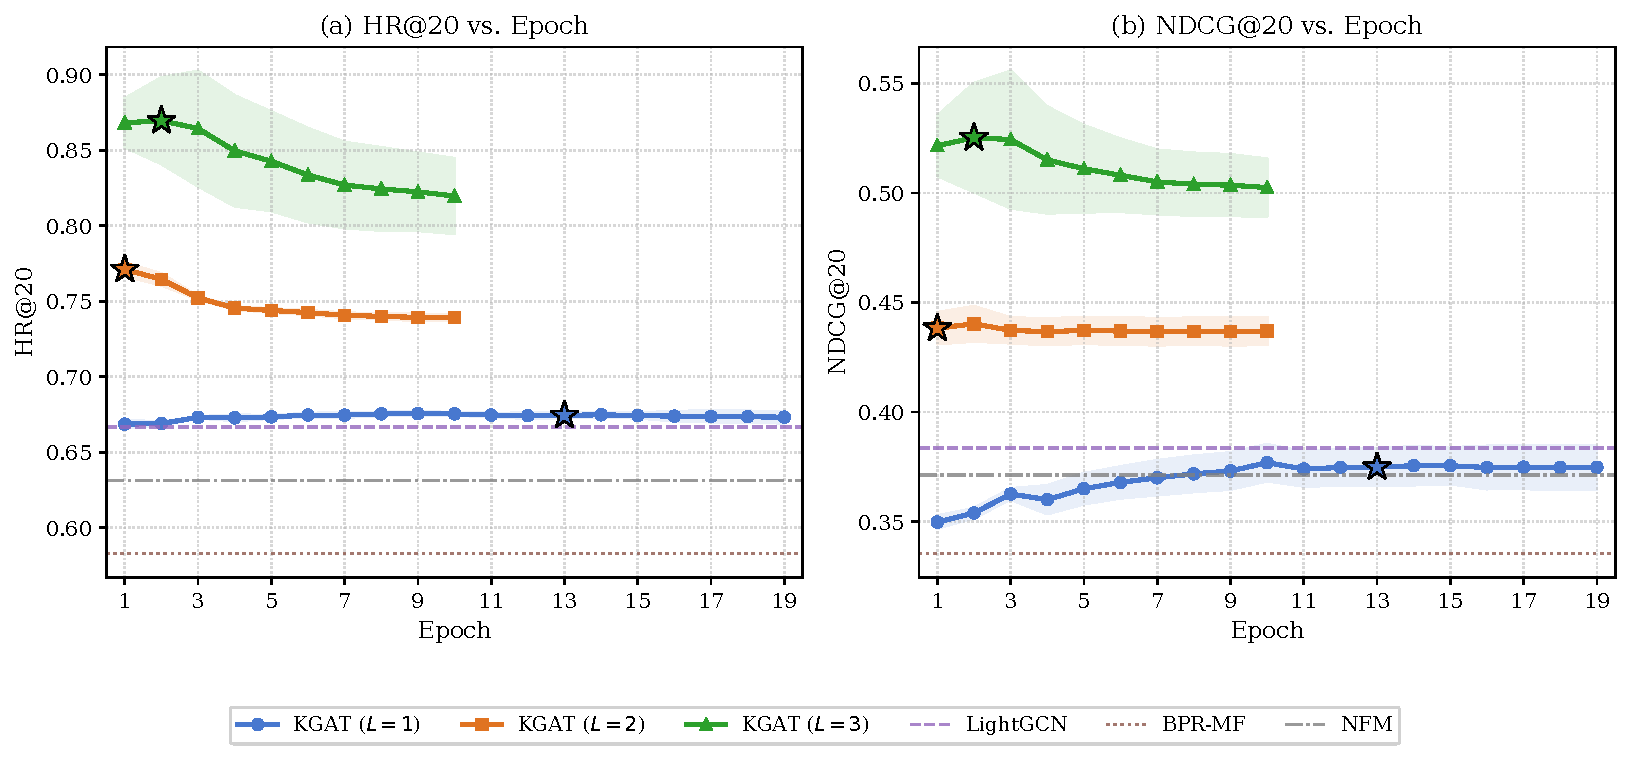
\includegraphics[width=0.92\linewidth]{figures/fig_training_curves.pdf}
  \caption{不同傳播深度 KGAT 模型的訓練過程比較（偶數 Epoch），含三條 Baseline 水平基線。}
  \label{fig:training_curves}
\end{figure}



\section{可解釋性評估 (Explainability Evaluation)}

本節基於 KGAT $L{=}3$ 模型（最佳效能模型），依研究設計，對 \textbf{100 位使用者} 進行解釋路徑萃取與 Fidelity 忠實度評估。使用者以均勻隨機抽樣方式從測試集中選取，篩選條件為該使用者在測試集中至少有一筆正樣本互動。解釋路徑的 Top-$K$ 萃取設定為 $K{=}3$，即每位使用者最多保留三條最高注意力分數的路徑。

\subsection*{解釋路徑覆蓋率與類型分析}

在 100 位使用者中，\textbf{60 位 (60\%)} 成功萃取出解釋路徑，40 位 (40\%) 無法萃取。無法萃取的主要原因為：在給定的最大跳數限制（$L{=}3$）下，使用者節點與其 Top-1 推薦物品之間不存在由高注意力邊連成的連通路徑。此結果表示，在本研究所採用的資料集、模型深度與路徑篩選設定下，並非所有推薦結果都能以顯式的結構路徑加以追蹤；部分預測可能更依賴嵌入空間中的分散式表示，而非可直接回溯的圖結構路徑。換言之，本研究觀察到的結構路徑解釋覆蓋率約為 60\%，但其是否為深層 GNN 推薦系統的一般性現象，仍有待後續研究在不同資料集與設定下進一步驗證。

從 60 位使用者中共萃取出 103 條解釋路徑，其類型分布如表~\ref{tab:path_types} 所示。

\begin{table}[htbp]
  \centering
  \caption{解釋路徑類型分布（103 條路徑，來自 60 位使用者）}
  \label{tab:path_types}
  \begin{tabular}{llcc}
    \toprule
    路徑結構 & 語意描述 & 數量 & 佔比 \\
    \midrule
    User $\to$ Recipe & 直接連接（已互動項目） & 23 & 22.3\% \\
    User $\to$ Recipe $\to$ User $\to$ Recipe & 協同過濾路徑 & 48 & 46.6\% \\
    User $\to$ Recipe $\to$ Entity $\to$ Recipe & KG 語意路徑 & 32 & 31.1\% \\
    \bottomrule
  \end{tabular}
\end{table}

協同過濾路徑（透過品味相近的使用者）佔比最高 (46.6\%)，其次為 KG 語意路徑（透過共同食材、菜系等屬性實體），直接連接路徑佔 22.3\%。值得關注的是各類型路徑的注意力分數差異極大：直接連接路徑的平均注意力分數高達 0.7907，而多跳路徑的分數則極為分散且低（協同過濾：0.0008，KG 語意：0.0002）。

\subsection{Fidelity 量化評估結果}

表~\ref{tab:fidelity_overall} 呈現了 60 位有效使用者的整體 Fidelity 統計結果。

\begin{table}[htbp]
  \centering
  \caption{Fidelity 量化評估結果（$n = 60$）}
  \label{tab:fidelity_overall}
  \begin{tabular}{l ccccc}
    \toprule
    指標 & Mean & Median & Std & Min & Max \\
    \midrule
    Fidelity$^+$ & \textbf{0.0711} & 0.0352 & 0.0772 & $-0.0023$ & \textbf{0.2415} \\
    Fidelity$^-$ & 0.0824 & \textbf{0.0019} & 0.1728 & $-0.0043$ & 0.6307 \\
    \bottomrule
  \end{tabular}
\end{table}

\begin{itemize}[leftmargin=2em]
  \item \textbf{Fidelity$^+$ 結果正向顯著：}93.3\% (56/60) 的路徑 $F^+ > 0$，顯示注意力權重確實標記了對預測有貢獻的邊。其中 33.3\% (20/60) 的路徑 $F^+ > 0.10$，具有顯著的影響力。
  \item \textbf{Fidelity$^-$ 中位數極低：}$F^-$ 的中位數僅為 0.0019，表明多數情況下「僅保留解釋路徑」即可幾乎完整維持原始預測。然而，Fidelity$^-$ 的平均值為 0.0824，標準差亦達 0.1728，表示不同樣本之間存在明顯差異。因此，整體中位數偏低並不代表所有解釋路徑皆具充分性，而較適合解讀為：在部分案例中，所萃取的路徑已能涵蓋模型決策的重要資訊，但其充分性仍受到路徑類型與個別樣本差異的明顯影響。
\end{itemize}

基於上述差異，若要進一步理解解釋品質，不能僅依賴整體統計量，仍需結合表~\ref{tab:fidelity_by_type} 所示之路徑類型分析，才能較完整地判讀不同解釋路徑的忠實度效能。

\subsection{路徑類型對忠實度的影響}

更深入的分析揭示了路徑類型對忠實度具有顯著影響，如表~\ref{tab:fidelity_by_type} 所示。

\begin{table}[htbp]
  \centering
  \caption{Fidelity 按路徑類型分析}
  \label{tab:fidelity_by_type}
  \begin{tabular}{l c cc l}
    \toprule
    路徑類型 & $n$ & Avg $F^+$ & Avg $F^-$ & 判斷 \\
    \midrule
    直接連接 & 23 & \textbf{0.1231} & $\bm{-0.0016}$ & 最佳忠實度 \\
    協同過濾 & 22 & 0.0521 & 0.0128 & 良好忠實度 \\
    KG 語意  & 15 & 0.0193 & \textbf{0.3134} & 部分忠實 \\
    \bottomrule
  \end{tabular}
\end{table}

此結果揭示了三個重要觀察：

\begin{enumerate}[leftmargin=2em]
  \item \textbf{直接連接路徑的忠實度最高：}Avg $F^+ = 0.1231$，$F^- \approx 0$，是最可信賴的解釋類型。這類路徑反映了使用者對特定食譜的顯著且直接的偏好。
  \item \textbf{協同過濾路徑具良好忠實度：}Avg $F^+ = 0.0521$，提供了「品味相似使用者」的有價值洞察，且 $F^-$ 極低。
  \item \textbf{KG 語意路徑的 $F^-$ 異常高：}Avg $F^- = 0.3134$，意味著「僅保留 KG 語意路徑」會造成約 31\% 的預測機率損失。這顯示此類路徑雖然在人類語意上往往合理，但未必足以單獨支撐模型的最終預測。此現象可能呼應圖資訊瓶頸假說~\cite{wu2020gib}——經過三層非線性傳播後，知識圖譜的結構資訊已高度壓縮進分散式嵌入中，而不再完全對應到單一可顯式追蹤的路徑。但本文並未直接設計驗證該假說之實驗，因此較適合將其視為一項值得後續追蹤的解釋方向，而非已被充分證實的結論。
\end{enumerate}

\subsection*{Fidelity 評估之方法限制}

值得注意的是，本研究所採用的 Fidelity 評估方法存在固有的限制。透過直接移除邊（$F^+$）或僅保留子圖（$F^-$）來進行重預測，可能導致圖結構的分佈偏移 (Distribution Shift)~\cite{agarwal2024fidelity}：模型在訓練階段從未見過如此「殘缺」的圖結構，因此在評估階段的預測行為可能偏離其正常運作模式。這意味著所觀察到的 $F^-$ 異常值，有可能部分來自於分佈偏移本身，而非純粹反映路徑的充分性不足。未來研究可考慮引入精煉反事實指標或基於重訓練 (Retrain) 的評估方式來緩解此問題。

除此之外，直接連接路徑、協同過濾路徑與 KG 語意路徑類型分別的樣本數皆不多，僅有 23、22、15 條，因此表~\ref{tab:fidelity_by_type} 的結果僅能作為初步參考，未來仍需擴大樣本數以進行更穩健的分析。

\subsection{案例分析}

以下展示三個具代表性的案例，分別對應直接連接、協同過濾與 KG 語意路徑，並輔以示意圖說明其忠實度差異：

\begin{figure}[htbp]
  \centering
  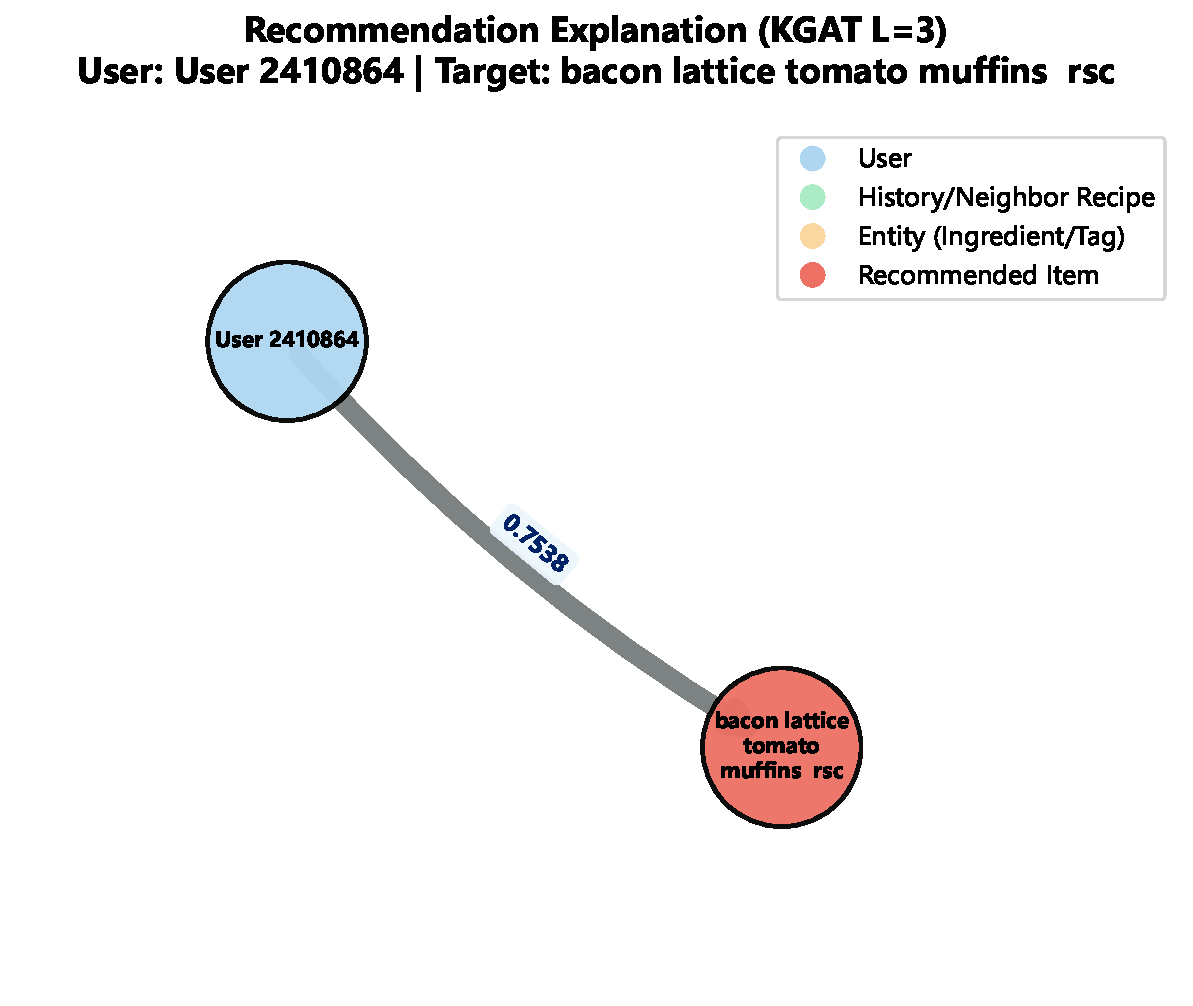
\includegraphics[width=0.8\linewidth]{figures/user_141540.pdf}
  \caption{案例 A：高忠實度的直接連接路徑示意圖 (User 2410864)}
  \label{fig:case_a}
\end{figure}

\textbf{案例 A：高忠實度的直接連接路徑（如圖~\ref{fig:case_a} 所示）。}
使用者 2410864 被推薦 ``bacon lattice tomato muffins''（預測機率 0.952），解釋路徑為使用者直接連向該食譜（注意力分數 0.767）。$F^+ = 0.2415$，$F^- = 0.0004$。移除此邊後預測信心大幅下降 24\%，證明此邊為預測的核心依據。

\begin{figure}[htbp]
  \centering
  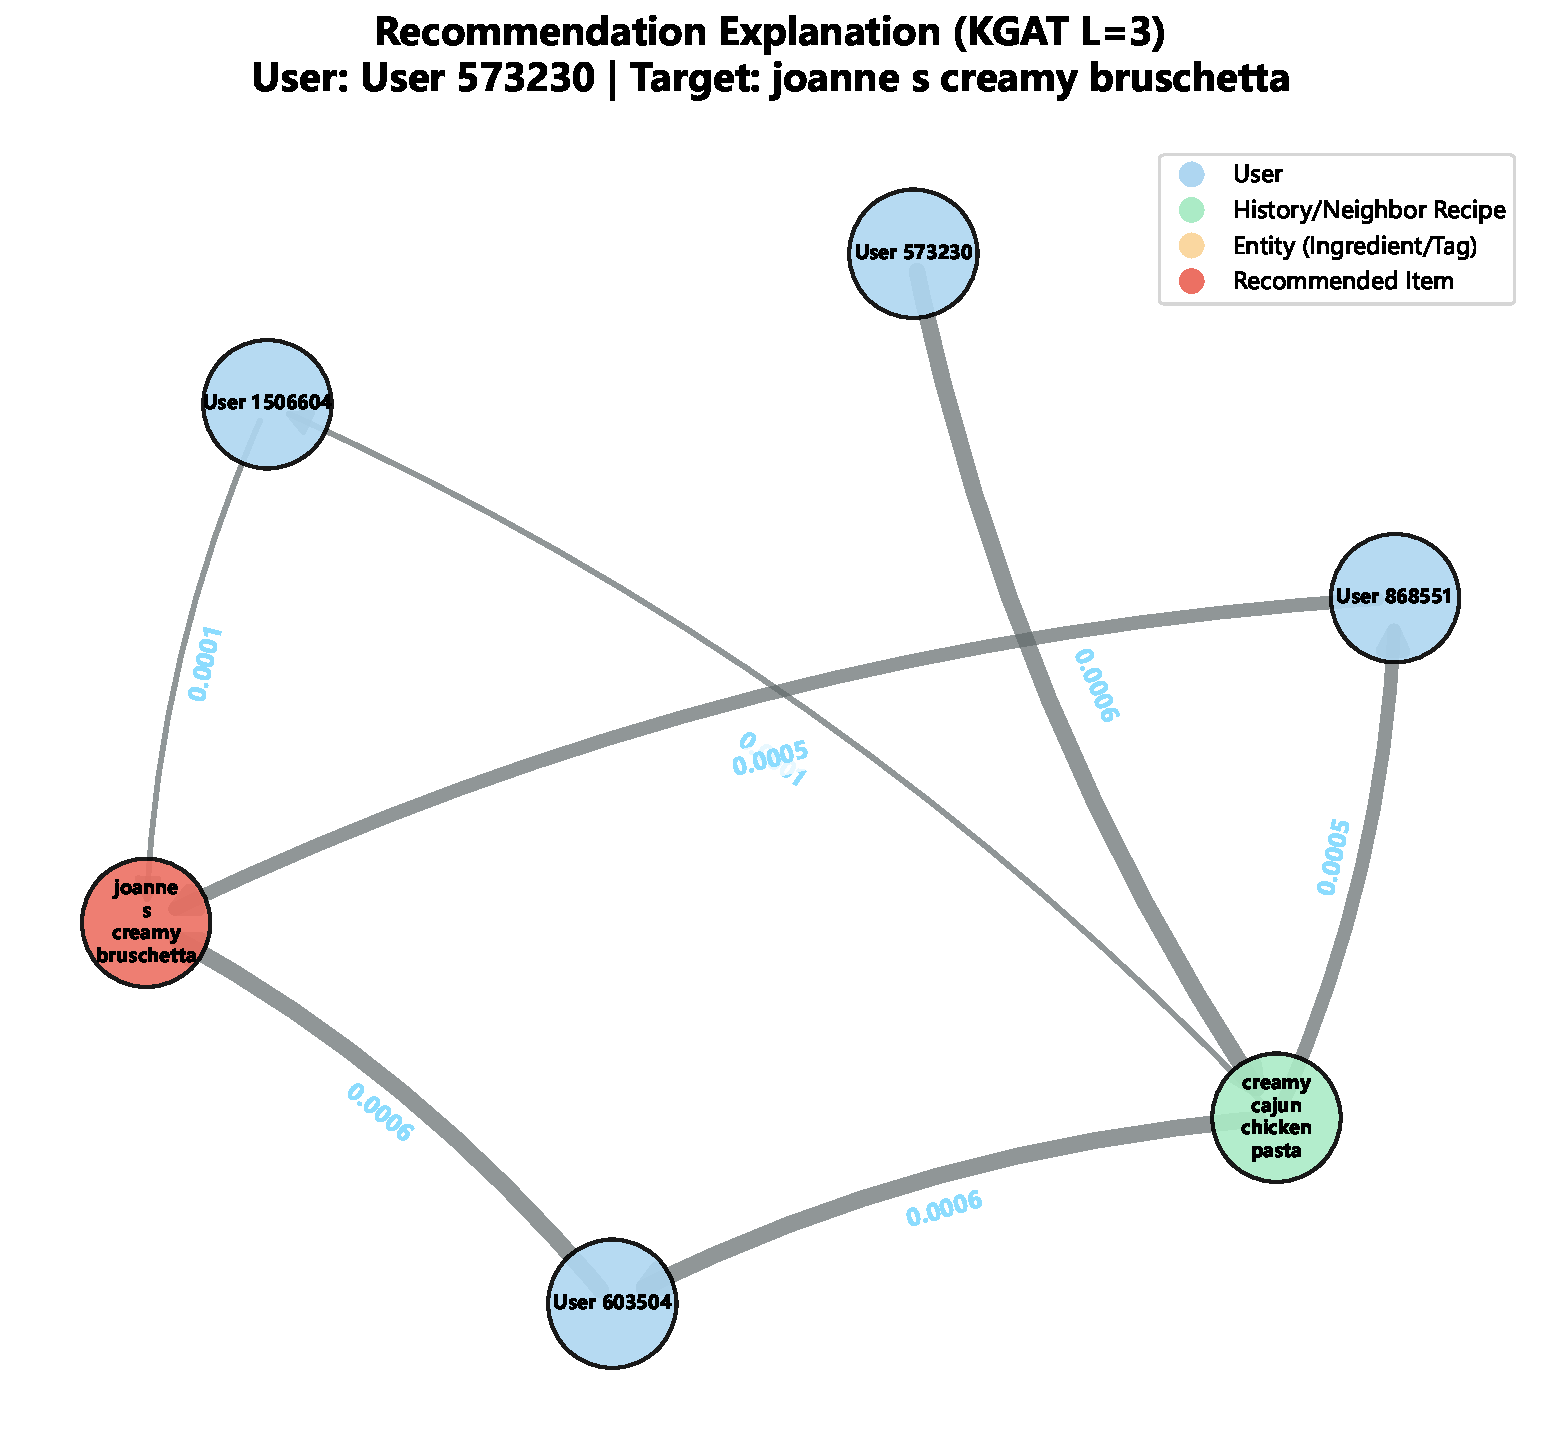
\includegraphics[width=0.8\linewidth]{figures/user_58074.pdf}
  \caption{案例 B：協同過濾路徑示意圖 (User 573230)}
  \label{fig:case_b}
\end{figure}

\textbf{案例 B：協同過濾路徑的知識發現（如圖~\ref{fig:case_b} 所示）。}
使用者 573230 被推薦 ``joanne's creamy bruschetta''（預測機率 0.952），解釋路徑為 User 573230 $\to$ creamy cajun chicken pasta $\to$ User 603504 $\to$ joanne's creamy bruschetta。儘管路徑注意力分數僅 0.0006，但 $F^+ = 0.2061$，$F^- = 0.0019$，顯示協同過濾路徑在整體預測中扮演關鍵角色。

\begin{figure}[htbp]
  \centering
  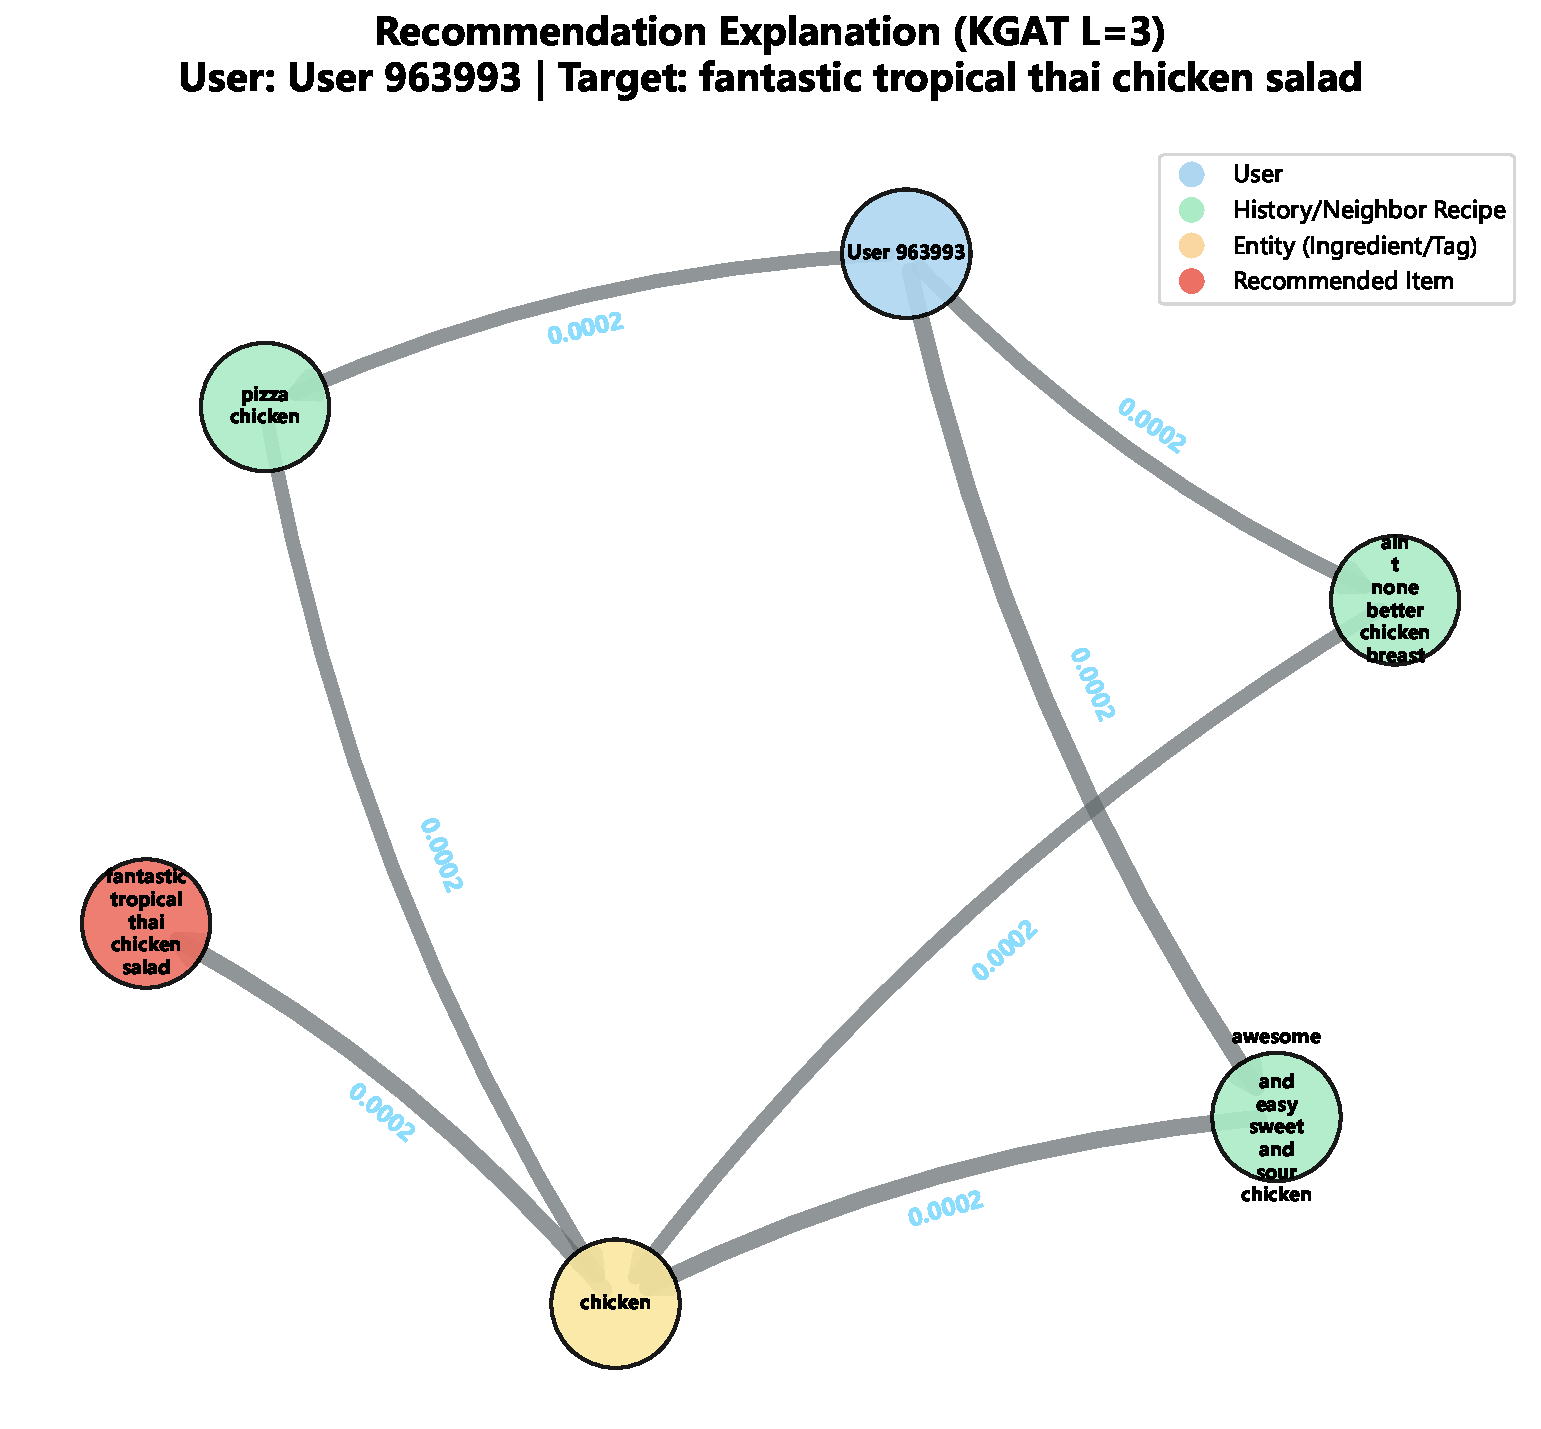
\includegraphics[width=0.8\linewidth]{figures/user_83279.pdf}
  \caption{案例 C：KG 語意路徑示意圖 (User 963993)}
  \label{fig:case_c}
\end{figure}

\textbf{案例 C：KG 語意路徑的侷限（如圖~\ref{fig:case_c} 所示）。}
使用者 963993 被推薦 ``fantastic tropical thai chicken salad''（預測機率 0.933），解釋路徑透過共同食材 ``chicken'' 建立聯繫。然而 $F^+ = -0.001$，$F^- = 0.5415$——移除路徑反而微幅提升預測，且僅保留路徑造成 54\% 的預測損失。此案例表明 KG 語意路徑雖然提供了直覺上合理的解釋，但並非模型預測的核心依據。

% !TeX root = ../main.tex

\chapter{結論與未來研究方向}

\section{研究結論}

本研究以知識圖譜注意力網路（KGAT）為核心，在 Food.com 食譜推薦資料集上進行效能評估與可解釋性分析。透過基準方法對比、深度比較、模組消融與 Fidelity 量化評估，本文對第一章所提出之三個研究問題提供了具一致趨勢的實證回答，並整理出若干與食譜知識圖譜特性相關的重要觀察。

需要指出的是，本文之結論主要建立於 Food.com 資料集、本文採用之評估協定，以及既定運算資源條件下的實驗結果。因此，下述發現較適合被理解為在本研究設定下所獲得之具體實證，而其跨資料集與跨設定的普適性，仍有待後續研究進一步驗證。

\subsection*{核心研究貢獻}

本研究的主要貢獻可歸納為三點：

\begin{enumerate}[leftmargin=2em]
  \item \textbf{深度效應之實證分析：}在食譜推薦領域觀察到 GNN 傳播深度與推薦效能之間存在顯著關聯，以從 $L{=}1$ 到 $L{=}3$ 的逐層消融實驗，量化了高階連接性的具體貢獻。
  \item \textbf{淺層知識圖譜資訊汙染現象之揭露與機制溯源：}發現並解釋了在 $L{=}1$ 淺層架構下，引入知識圖譜反而導致效能下降的「資訊汙染」現象。此反直覺發現填補了傳統認知中「引入知識必然有益」的盲點，並提出了具體的機制解釋——高連接度樞紐節點在淺層聚合中稀釋協同過濾訊號。
  \item \textbf{深層模型之端到端 Fidelity 驗證框架：}建立了一套從注意力路徑萃取到忠實度量化的完整可解釋性驗證管線，並在最佳效能的 $L{=}3$ 模型上對 103 條解釋路徑進行了初步 Fidelity 評估，揭露了 KG 語意路徑的充分性危機（$F^- = 0.3134$）——即人類語意上合理的解釋路徑，在數學上不足以支撐模型的預測信心。
\end{enumerate}

\subsection*{回應 RQ1：圖神經網路深度與知識圖譜整合如何影響推薦效能？}

實驗結果指出\textbf{訊息傳播深度是決定推薦效能的關鍵因素}。三層架構 ($L{=}3$) 的 KGAT 在所有指標上全面超越基準方法，其 HR@20 達到 0.9368，較最強的 Baseline (LightGCN, 0.6717) 提升了 39.5\%，NDCG@20 達到 0.5891，提升幅度更高達 52.7\%。深度每增加一層，HR@20 皆呈現顯著提升，充分支持在知識圖譜推薦場景中，二跳與三跳的高階連接性蘊含了極為關鍵的協同過濾訊號。

同時，消融實驗揭露了一個重要的反直覺發現：在淺層架構 ($L{=}1$) 下，移除知識圖譜後 HR@20 反而從 0.7910 提升至 0.8621（+9.0\%），NDCG@20 從 0.4440 提升至 0.5255（+18.4\%）。我們推測此現象的主因在於食譜知識圖譜中大量高連接度的樞紐實體節點——例如「chicken」或「breakfast」等常見食材與標籤——在 $L{=}1$ 的單跳聚合中，將高度泛化的特徵無差別地灌注至食譜嵌入，嚴重稀釋了純粹的協同過濾訊號。知識圖譜的引入需要搭配足夠的網路深度，使模型能透過多跳傳播逐步篩選有價值的語意關聯，同時以注意力機制抑制雜訊。

\subsection*{回應 RQ2：不同傳播深度下，模型的訓練行為與泛化能力有何差異？}

從附錄~\ref{app:training_log} 所呈現的 KGAT $L{=}3$ 模型三個完整 Epoch 訓練歷程來看，模型在訓練初期便展現了極快的收斂速度：第 1 個 Epoch 結束時，HR@20 已達到 0.8906，至第 3 個 Epoch 微幅上升至 0.9185，增幅僅 3.1\%。配合 NDCG@20 從 0.5406 上升至 0.5687（+5.2\%）來看，深層模型的核心效能在前三個 Epoch 內的增長空間已顯著收窄，可能預示著更長訓練週期下會面臨過擬合的風險。

此外，為進一步驗證模型在更長訓練週期的行為，本研究在偶數 Epoch 的模型檢查點上進行了額外的完整指標評估（詳見附錄~\ref{app:ablation_data}）。在此擴展評估窗口中，$L{=}3$ 的 HR@20 從 E2 的 0.9120 持續上升至 E10 的 0.9368，但增幅急劇趨緩（E2$\to$E10 僅增加 2.7\%，而 $L{=}1$ 在相同區間增加 6.2\%），再次印證深層模型的核心效能在訓練初期便已大致形成。

\subsection*{回應 RQ3：基於注意力機制的解釋路徑是否忠實地反映了模型的決策邏輯？}

依研究設計，抽取 100 位使用者、其中 60 位成功萃取解釋路徑進行初步忠實度評估，本研究驗證了注意力解釋路徑展現出\textbf{方向一致但程度差異化的忠實度}：

\begin{itemize}[leftmargin=2em]
  \item 93.3\% 的路徑 $F^+ > 0$，平均 $F^+ = 0.0711$，顯示注意力權重確實標記了對預測有貢獻的邊。
  \item 直接連接路徑的忠實度最高 (Avg $F^+ = 0.1231$, $F^- \approx 0$)，可被視為高可信度的解釋類型。
  \item 協同過濾路徑同樣具備良好忠實度 (Avg $F^+ = 0.0521$, $F^- = 0.0128$)，驗證了群體品味訊號的決策貢獻。
  \item 然而，KG 語意路徑的 $F^- = 0.3134$ 異常偏高，意味著「僅保留 KG 語意路徑」會導致約 31\% 的預測機率損失。我們推測，經過三層非線性訊息傳播後，知識圖譜的結構與語意資訊已被高度壓縮至節點的分散式嵌入向量中，使得單一的顯式路徑無法涵蓋模型實際依賴的全部特徵。此發現可能呼應圖資訊瓶頸假說~\cite{wu2020gib}，並顯示基於注意力的內在可解釋性在深層 GNN 中可能存在結構性的侷限。
  \item 解釋路徑的覆蓋率觀察到約 60\%，約四成的推薦無法透過 Top-$K$ 注意力路徑進行解釋，進一步佐證了分散式嵌入在深層模型決策中的主導地位。
\end{itemize}

\section{研究限制}

本研究仍存在以下限制，需於未來工作中加以改善：

\begin{enumerate}[leftmargin=2em]
  \item \textbf{訓練資源與實驗規模：}受限於深層模型所需的運算時間與記憶體成本，KGAT 目前尚未如 Baseline 模型般進行多次獨立重複運行，且完整指標評估主要集中於偶數 Epoch。此一設定使本文較難充分評估模型效能的統計穩定性，也限制了對長期訓練行為的完整觀察。
  \item \textbf{實驗比較口徑未完全對稱：}Baseline 模型採兩次獨立運行後取最佳 Epoch 平均，而 KGAT 則是在既定資源條件下，以一次訓練過程中的最佳觀察值進行報告。雖然本文已明確說明其原因，但此差異仍意味著 KGAT 與 Baseline 之間的比較應視為在特定條件下的實證觀察，而非已完全排除訓練成本與隨機性的最終結論。
  \item \textbf{單一資料集驗證：}本研究僅在 Food.com 食譜推薦資料集上進行驗證。食譜領域知識圖譜的特殊結構（如高頻樞紐食材節點）可能放大了淺層「資訊汙染」效應。因此，本文所觀察到的深度效應與知識圖譜整合效果，是否能推廣至其他領域資料集，仍有待交叉驗證。
  \item \textbf{評估協定的侷限：}本文採用 Leave-one-out 評估，並為每筆正樣本隨機抽取 100 個負樣本形成候選清單。此作法有助於控制評估成本與比較條件，但也使本文所報告之 HR 與 NDCG 數值主要適合用於相同協定下的相對比較，不宜直接與 full-ranking 或不同負樣本抽樣設定的研究進行絕對值對照。
  \item \textbf{可解釋性分析之樣本有限：}雖然可解釋性評估初始抽取了 100 位使用者，但實際成功萃取出解釋路徑者為 60 位，因此 Fidelity 統計係建立於有效樣本子集合之上。這代表本文所觀察到的忠實度分布，主要反映「可成功萃取路徑之樣本」的特性，而不必然能代表所有推薦結果。
  \item \textbf{Fidelity 指標的固有限制：}本研究採用的傳統 Fidelity 評估透過直接移除或保留邊進行重預測，可能引發資料分佈偏移 (Distribution Shifts)，使評估結果存在一定程度的失真~\cite{agarwal2024fidelity}。因此，本文對解釋路徑充分性與必要性的判讀，仍需結合此方法限制一併理解。
\end{enumerate}

\section{未來研究方向}

基於本研究的發現與上述限制，以下提出四個值得深入探索的未來研究方向：

\begin{enumerate}[leftmargin=2em]
  \item \textbf{擴展訓練規模與重複驗證：}最優先的後續工作為增加 KGAT 模型的訓練 Epoch 數，並進行至少兩次以上的獨立重複運行，報告各指標的平均值與標準差，以確認效能的統計穩定性。同時，引入 DropEdge~\cite{rong2020dropedge}、Message Dropout 或 Early Stopping 等正則化策略，緩解深層模型的訓練不穩定與過擬合風險，進一步挖掘深層架構的潛力。

  \item \textbf{探究 KG 語意路徑充分性偏低的深層機制：}本研究發現 KG 語意路徑的 $F^-$ 顯著高於其他路徑類型。未來研究可從圖資訊瓶頸 (Graph Information Bottleneck)~\cite{wu2020gib} 的角度，分析模型在深層傳播後是否已將 KG 結構資訊壓縮進了分散式嵌入中，從而使得僅保留顯式 KG 路徑不足以支撐預測。此外，可嘗試引入精煉反事實指標 (Refined Counterfactual Metrics) 以緩解傳統 Fidelity 計算中的分佈偏移問題~\cite{agarwal2024fidelity}。

  \item \textbf{跨資料集與跨領域驗證：}為增強研究結論的泛化性，未來應在其他領域的知識圖譜推薦資料集（如 Amazon-Book、Yelp2018 等）上進行交叉驗證，檢驗深度效應、淺層 KG 資訊汙染與 KG 語意路徑充分性危機等結論是否具備跨領域的普適性。

  \item \textbf{消融實驗之系統性擴展：}目前的消融實驗（w/o Attention、w/o KG）僅在 $L{=}1$ 層級進行模組拆解。未來可將消融拓展至 $L{=}2$、$L{=}3$ 等深層配置，觀察注意力機制與知識圖譜在不同深度下的邊際貢獻是否存在質變，以建構更完整的元件貢獻圖像。
\end{enumerate}


% 參考文獻
% References
\refmatter
\bibliographystyle{abbrv}
\bibliography{back/references}

% 附錄
% Appendices
% !TeX root = ../main.tex

\appendix{A}{實驗日誌與訓練細節}
\refstepcounter{chapter}
\label{app:training_log}

\section{KGAT ($L{=}3$) 訓練過程}

表~\ref{tab:kgat_l3_training} 呈現了 KGAT $L{=}3$ 模型的完整訓練過程，包含每個 Epoch 的損失值與評估指標。

\begin{table}[htbp]
  \centering
  \footnotesize
  \setlength{\tabcolsep}{3.5pt}
  \caption{KGAT ($L{=}3$) 訓練過程詳細數據}
  \label{tab:kgat_l3_training}
  \begin{tabular}{c c ccc ccc ccc}
    \toprule
    Epoch & Loss & HR@10 & HR@20 & HR@50 & Prec@10 & Prec@20 & Prec@50 & NDCG@10 & NDCG@20 & NDCG@50 \\
    \midrule
    1 & 0.2823 & 0.7538 & 0.8906 & 0.9859 & 0.0754 & 0.0445 & 0.0197 & 0.5059 & 0.5406 & 0.5601 \\
    2 & 0.2190 & 0.7788 & 0.9097 & 0.9890 & 0.0779 & 0.0455 & 0.0198 & 0.5271 & 0.5604 & 0.5766 \\
    3 & 0.2026 & \textbf{0.7916} & \textbf{0.9185} & \textbf{0.9897} & \textbf{0.0792} & \textbf{0.0459} & \textbf{0.0198} & \textbf{0.5364} & \textbf{0.5687} & \textbf{0.5833} \\
    \bottomrule
  \end{tabular}
\end{table}

\section{Baseline 模型訓練過程}

每個 Baseline 模型均執行兩次獨立運行，取最佳 Epoch 之平均值作為報告結果。以下呈現各 Baseline 最佳 Epoch 的詳細數據。

\begin{table}[H]
  \centering
  \footnotesize
  \setlength{\tabcolsep}{4.5pt}
  \caption{BPR-MF 兩次運行最佳 Epoch 結果}
  \label{tab:bprmf_runs}
  \begin{tabular}{c ccc ccc ccc}
    \toprule
    Run & HR@10 & HR@20 & HR@50 & Prec@10 & Prec@20 & Prec@50 & NDCG@10 & NDCG@20 & NDCG@50 \\
    \midrule
    2 (E10) & 0.4544 & 0.5671 & 0.7319 & 0.0454 & 0.0284 & 0.0146 & 0.2982 & 0.3266 & 0.3593 \\
    3 (E10) & 0.4562 & 0.5680 & 0.7328 & 0.0456 & 0.0284 & 0.0147 & 0.2998 & 0.3280 & 0.3608 \\
    \midrule
    Average & 0.4553 & 0.5675 & 0.7324 & 0.0455 & 0.0284 & 0.0146 & 0.2990 & 0.3273 & 0.3600 \\
    \bottomrule
  \end{tabular}
\end{table}

\begin{table}[H]
  \centering
  \footnotesize
  \setlength{\tabcolsep}{4.5pt}
  \caption{LightGCN 兩次運行最佳 Epoch 結果}
  \label{tab:lightgcn_runs}
  \begin{tabular}{c ccc ccc ccc}
    \toprule
    Run & HR@10 & HR@20 & HR@50 & Prec@10 & Prec@20 & Prec@50 & NDCG@10 & NDCG@20 & NDCG@50 \\
    \midrule
    2 (E2) & 0.5371 & 0.6718 & 0.8560 & 0.0537 & 0.0336 & 0.0171 & 0.3516 & 0.3856 & 0.4223 \\
    3 (E2) & 0.5366 & 0.6716 & 0.8562 & 0.0537 & 0.0336 & 0.0171 & 0.3518 & 0.3859 & 0.4227 \\
    \midrule
    Average & 0.5369 & 0.6717 & 0.8561 & 0.0537 & 0.0336 & 0.0171 & 0.3517 & 0.3858 & 0.4225 \\
    \bottomrule
  \end{tabular}
\end{table}

\begin{table}[H]
  \centering
  \footnotesize
  \setlength{\tabcolsep}{4.5pt}
  \caption{NFM 兩次運行最佳 Epoch 結果}
  \label{tab:nfm_runs}
  \begin{tabular}{c ccc ccc ccc}
    \toprule
    Run & HR@10 & HR@20 & HR@50 & Prec@10 & Prec@20 & Prec@50 & NDCG@10 & NDCG@20 & NDCG@50 \\
    \midrule
    2 (E3) & 0.3507 & 0.4521 & 0.6788 & 0.0351 & 0.0226 & 0.0136 & 0.2277 & 0.2531 & 0.2976 \\
    3 (E6) & 0.3471 & 0.4430 & 0.6731 & 0.0347 & 0.0222 & 0.0135 & 0.2350 & 0.2590 & 0.3041 \\
    \midrule
    Average & 0.3489 & 0.4476 & 0.6760 & 0.0349 & 0.0224 & 0.0135 & 0.2314 & 0.2560 & 0.3008 \\
    \bottomrule
  \end{tabular}
\end{table}

% !TeX root = ../main.tex

\appendix{B}{消融實驗偶數 Epoch 完整數據}
\refstepcounter{chapter}
\label{app:ablation_data}

\section{Full KGAT ($L{=}1$) 偶數 Epoch 訓練過程}

\begin{table}[H]
  \centering
  \footnotesize
  \setlength{\tabcolsep}{3.5pt}
  \caption{Full KGAT ($L{=}1$) 偶數 Epoch 評估結果}
  \label{tab:full_kgat_detail}
  \begin{tabular}{c c ccc ccc ccc}
    \toprule
    Epoch & Loss & HR@10 & HR@20 & HR@50 & Prec@10 & Prec@20 & Prec@50 & NDCG@10 & NDCG@20 & NDCG@50 \\
    \midrule
    2 & 0.4167 & 0.5980 & 0.7449 & 0.9051 & 0.0598 & 0.0372 & 0.0181 & 0.3661 & 0.4033 & 0.4353 \\
    4 & 0.3931 & 0.6176 & 0.7690 & 0.9225 & 0.0618 & 0.0385 & 0.0184 & 0.3848 & 0.4232 & 0.4540 \\
    6 & 0.3814 & 0.6284 & 0.7801 & 0.9316 & 0.0628 & 0.0390 & 0.0186 & 0.3961 & 0.4345 & 0.4650 \\
    8 & 0.3757 & 0.6341 & 0.7862 & 0.9372 & 0.0634 & 0.0393 & 0.0187 & 0.4015 & 0.4400 & 0.4704 \\
    10 & 0.3717 & \textbf{0.6383} & \textbf{0.7910} & \textbf{0.9404} & \textbf{0.0638} & \textbf{0.0396} & \textbf{0.0188} & \textbf{0.4054} & \textbf{0.4440} & \textbf{0.4742} \\
    \bottomrule
  \end{tabular}
\end{table}

\section{w/o Attention ($L{=}1$) 偶數 Epoch 訓練過程}

\begin{table}[H]
  \centering
  \footnotesize
  \setlength{\tabcolsep}{3.5pt}
  \caption{w/o Attention ($L{=}1$) 偶數 Epoch 評估結果}
  \label{tab:wo_attn_detail}
  \begin{tabular}{c c ccc ccc ccc}
    \toprule
    Epoch & Loss & HR@10 & HR@20 & HR@50 & Prec@10 & Prec@20 & Prec@50 & NDCG@10 & NDCG@20 & NDCG@50 \\
    \midrule
    2 & 0.4342 & 0.6029 & 0.7211 & 0.8943 & 0.0603 & 0.0361 & 0.0179 & 0.4002 & 0.4302 & 0.4640 \\
    4 & 0.4135 & 0.6277 & 0.7452 & 0.9080 & 0.0628 & 0.0373 & 0.0182 & 0.4241 & 0.4539 & 0.4857 \\
    6 & 0.4032 & 0.6418 & 0.7613 & 0.9113 & 0.0642 & 0.0381 & 0.0182 & 0.4392 & 0.4696 & 0.4990 \\
    8 & 0.3953 & 0.6521 & 0.7727 & 0.9147 & 0.0652 & 0.0386 & 0.0183 & 0.4496 & 0.4802 & 0.5081 \\
    10 & 0.3901 & \textbf{0.6592} & \textbf{0.7800} & \textbf{0.9137} & \textbf{0.0659} & \textbf{0.0390} & \textbf{0.0183} & \textbf{0.4569} & \textbf{0.4875} & \textbf{0.5140} \\
    \bottomrule
  \end{tabular}
\end{table}

\section{w/o KG ($L{=}1$) 偶數 Epoch 訓練過程}

\begin{table}[H]
  \centering
  \footnotesize
  \setlength{\tabcolsep}{3.5pt}
  \caption{w/o KG ($L{=}1$) 偶數 Epoch 評估結果}
  \label{tab:wo_kg_detail}
  \begin{tabular}{c c ccc ccc ccc}
    \toprule
    Epoch & Loss & HR@10 & HR@20 & HR@50 & Prec@10 & Prec@20 & Prec@50 & NDCG@10 & NDCG@20 & NDCG@50 \\
    \midrule
    2 & 0.4448 & 0.6470 & 0.7787 & 0.9279 & 0.0647 & 0.0389 & 0.0186 & 0.4275 & 0.4608 & 0.4908 \\
    4 & 0.4099 & 0.6842 & 0.8179 & 0.9493 & 0.0684 & 0.0409 & 0.0190 & 0.4595 & 0.4933 & 0.5199 \\
    6 & 0.3876 & 0.6995 & 0.8367 & 0.9589 & 0.0700 & 0.0418 & 0.0192 & 0.4722 & 0.5070 & 0.5317 \\
    8 & 0.3742 & 0.7130 & 0.8522 & 0.9634 & 0.0713 & 0.0426 & 0.0193 & 0.4833 & 0.5185 & 0.5411 \\
    10 & 0.3679 & \textbf{0.7225} & \textbf{0.8621} & \textbf{0.9658} & \textbf{0.0723} & \textbf{0.0431} & \textbf{0.0193} & \textbf{0.4901} & \textbf{0.5255} & \textbf{0.5465} \\
    \bottomrule
  \end{tabular}
\end{table}

\section{KGAT ($L{=}2$) 偶數 Epoch 訓練過程}

\begin{table}[H]
  \centering
  \footnotesize
  \setlength{\tabcolsep}{3.5pt}
  \caption{KGAT ($L{=}2$) 偶數 Epoch 評估結果}
  \label{tab:depth2_detail}
  \begin{tabular}{c c ccc ccc ccc}
    \toprule
    Epoch & Loss & HR@10 & HR@20 & HR@50 & Prec@10 & Prec@20 & Prec@50 & NDCG@10 & NDCG@20 & NDCG@50 \\
    \midrule
    2 & 0.2889 & 0.6875 & 0.8369 & 0.9737 & 0.0688 & 0.0418 & 0.0195 & 0.4452 & 0.4830 & 0.5108 \\
    4 & 0.2662 & 0.7080 & 0.8564 & 0.9752 & 0.0708 & 0.0428 & 0.0195 & 0.4617 & 0.4993 & 0.5235 \\
    6 & 0.2551 & 0.7192 & 0.8666 & 0.9771 & 0.0719 & 0.0433 & 0.0195 & 0.4714 & 0.5087 & 0.5312 \\
    8 & 0.2500 & 0.7250 & 0.8725 & 0.9772 & 0.0725 & 0.0436 & 0.0195 & 0.4758 & 0.5132 & 0.5346 \\
    10 & 0.2476 & \textbf{0.7282} & \textbf{0.8766} & \textbf{0.9775} & \textbf{0.0728} & \textbf{0.0438} & \textbf{0.0196} & \textbf{0.4788} & \textbf{0.5165} & \textbf{0.5371} \\
    \bottomrule
  \end{tabular}
\end{table}

\section{KGAT ($L{=}3$) 偶數 Epoch 訓練過程}

\begin{table}[H]
  \centering
  \footnotesize
  \setlength{\tabcolsep}{3.5pt}
  \caption{KGAT ($L{=}3$) 偶數 Epoch 評估結果}
  \label{tab:depth3_detail}
  \begin{tabular}{c c ccc ccc ccc}
    \toprule
    Epoch & Loss & HR@10 & HR@20 & HR@50 & Prec@10 & Prec@20 & Prec@50 & NDCG@10 & NDCG@20 & NDCG@50 \\
    \midrule
    2 & 0.2189 & 0.7790 & 0.9120 & 0.9899 & 0.0779 & 0.0456 & 0.0198 & 0.5269 & 0.5608 & 0.5767 \\
    4 & 0.1941 & 0.7991 & 0.9241 & 0.9905 & 0.0799 & 0.0462 & 0.0198 & 0.5445 & 0.5764 & 0.5900 \\
    6 & 0.1838 & 0.8130 & 0.9324 & 0.9906 & 0.0813 & 0.0466 & 0.0198 & 0.5543 & 0.5848 & 0.5967 \\
    8 & 0.1786 & 0.8185 & 0.9348 & 0.9905 & 0.0818 & 0.0467 & 0.0198 & 0.5573 & 0.5871 & 0.5984 \\
    10 & 0.1768 & \textbf{0.8225} & \textbf{0.9368} & \textbf{0.9901} & \textbf{0.0822} & \textbf{0.0468} & \textbf{0.0198} & \textbf{0.5599} & \textbf{0.5891} & \textbf{0.6000} \\
    \bottomrule
  \end{tabular}
\end{table}

% !TeX root = ../main.tex

\appendix{C}{知識圖預處理與超級節點過濾清單}
\refstepcounter{chapter}
\label{app:preprocessing}

在構建食譜知識圖時，少數出現頻率極高的節點（如常見的調味料或無區別性的通用標籤）會成為結構中的超級節點（Hub Nodes）。在圖神經網路的訊息傳遞過程中，這些超級節點會將高度同質化的資訊無差別地廣播給大量不相關的食譜，導致協同過濾訊號被嚴重稀釋，這也是發生淺層網路「資訊污染」現象的可能原因之一。

為維持知識圖中語意關聯的鑑別度並控制運算複雜度，本研究在預處理階段針對食材與標籤進行了分佈分析，設定閾值以過濾部分極高頻的超級節點。為確保本實驗的設計細節透明與可重複性（Reproducibility），具體的過濾名單詳列於本附錄中供參考。

\section{食材 (Ingredients) 噪音與過濾清單}

食材過濾清單由兩部分聯集而成：一是根據先驗常識手動加入的基礎調味料（Base Noise）；二是統計所有食譜後，出現頻率位居前 0.5\% 或前十名的高頻食材。此過濾邏輯總共排除了 74 個高頻食材實體：

\begin{itemize}[leftmargin=2em]
  \item \textbf{基礎過濾清單 (Base Noise):} salt, water, oil, sugar, all-purpose flour, butter, eggs, black pepper, garlic, onions, vanilla, baking soda, baking powder.
  \item \textbf{高頻過濾清單 (Top 0.5\%):} carrot, red onion, onion, unsalted butter, green onion, zucchini, ground beef, ground cinnamon, cinnamon, honey, cream cheese, mayonnaise, fresh parsley, potatoes, celery, red bell pepper, tomatoes, parsley, dijon mustard, orange juice, cayenne pepper, margarine, olive oil, soy sauce, dried oregano, vegetable oil, garlic clove, garlic powder, worcestershire sauce, flour, carrots, powdered sugar, paprika, lemon juice, kosher salt, cheddar cheese, milk, garlic cloves, sour cream, chili powder, nutmeg, fresh lemon juice, fresh ground black pepper, mozzarella cheese, cornstarch, parmesan cheese, green onions, heavy cream, chicken broth, raisins, granulated sugar, brown sugar, vanilla extract, extra virgin olive oil, bacon, walnuts, pecans, salt and pepper, ground cumin, pepper, egg.
\end{itemize}

\section{標籤 (Tags) 噪音與過濾清單}

針對食譜標籤，考量標籤的種類總數相對較少（Total unique tags: 552），本研究直接剃除出現頻率最高的前 50 個標籤。這些標籤大多表示製作時間長短、適用場合、或是極度通用的食譜分類（對區別食譜特徵的貢獻極低），完整的過濾清單如下：

\begin{itemize}[leftmargin=2em]
  \item \textbf{高頻標籤過濾清單 (Top 50):} 4-hours-or-less, course, 15-minutes-or-less, comfort-food, desserts, oven, time-to-make, lunch, occasion, equipment, dietary, low-saturated-fat, preparation, holiday-event, healthy-2, low-carb, inexpensive, poultry, north-american, side-dishes, 3-steps-or-less, low-fat, vegetables, 5-ingredients-or-less, taste-mood, easy, 30-minutes-or-less, 60-minutes-or-less, european, low-sodium, low-cholesterol, low-protein, eggs-dairy, pasta-rice-and-grains, presentation, vegetarian, dinner-party, beginner-cook, fruit, kid-friendly, low-in-something, american, main-ingredient, for-1-or-2, healthy, low-calorie, main-dish, cuisine, number-of-servings, meat.
\end{itemize}


\end{document}
